% Appendix A

\chapter{1-D Memristor Simulations} % Main appendix title

%\label{AppendixA} % For referencing this appendix elsewhere, use \ref{AppendixA}

%\lhead{Appendix A. \emph{Appendix Title Here}} % This is for the header on each page - perhaps a shortened title


\section{1-D Memristor (Cross section 2)}

\begin{landscape}
\begin{figure}[!htp]
\centering
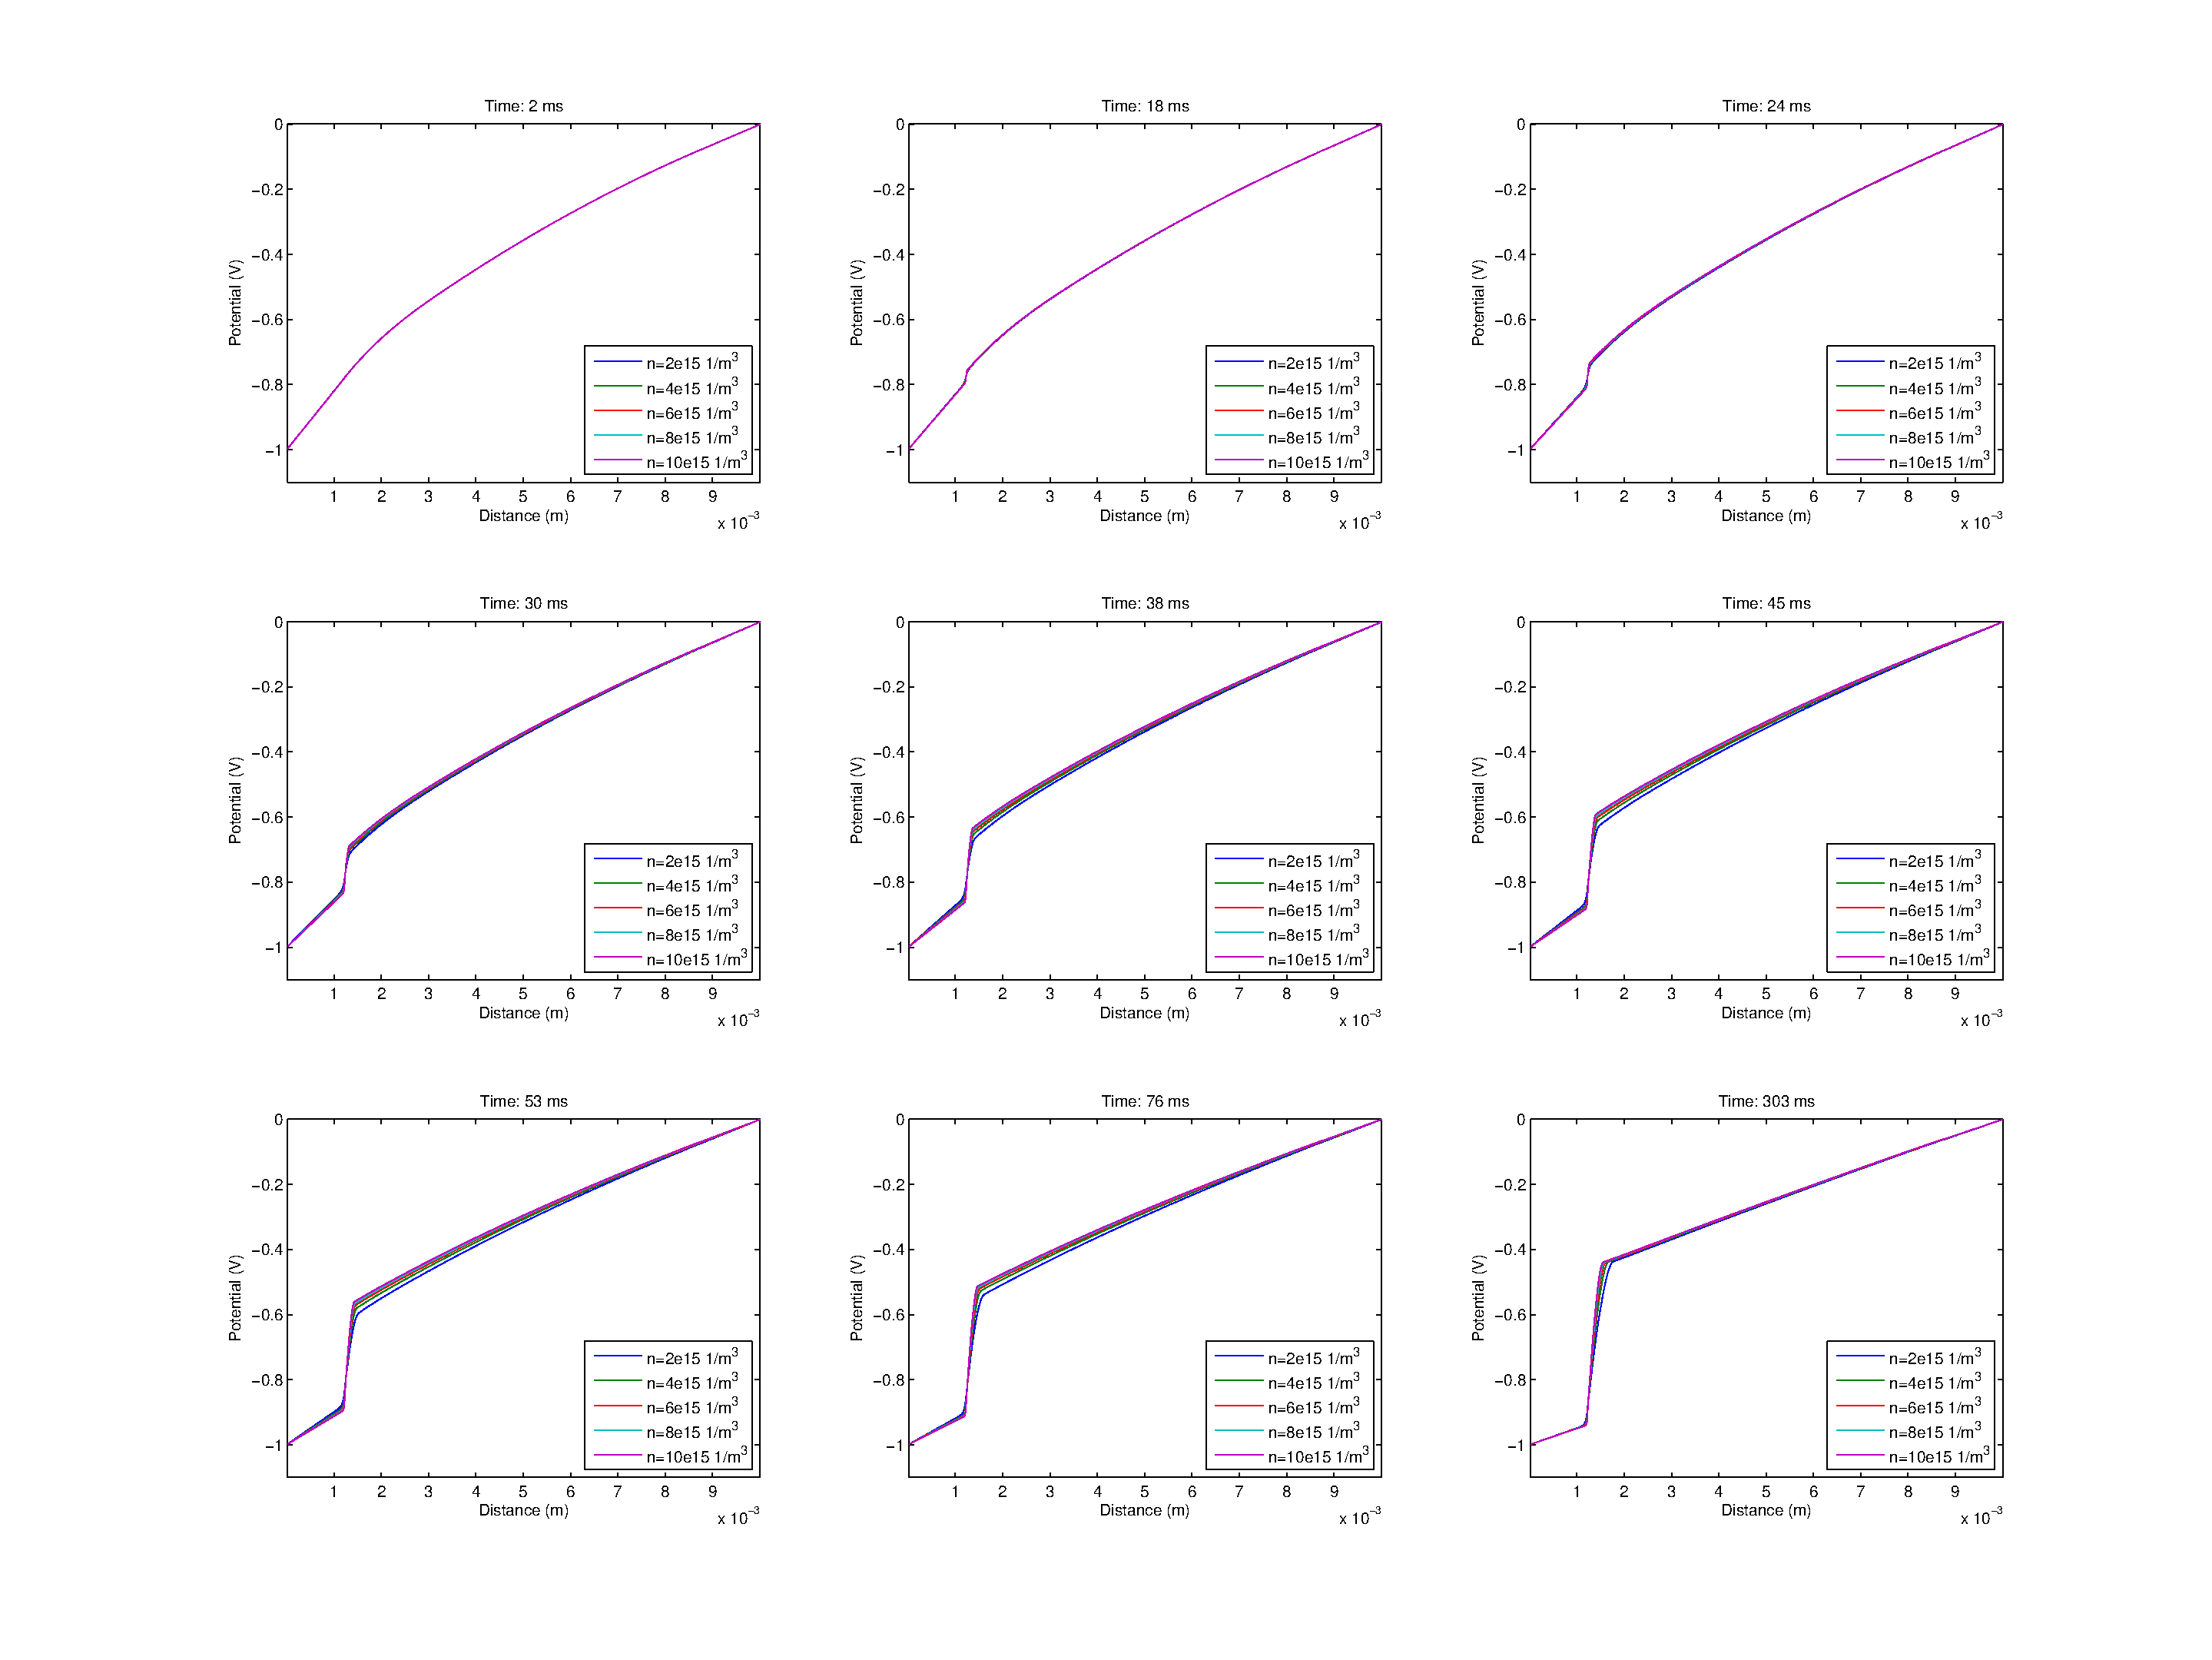
\includegraphics[scale=0.40]{Ex5V_Time1}
\caption{1-D Memristor potential distribution over time} 
\label{MemV}
\end{figure}
\end{landscape}


\begin{landscape}
\begin{figure}[!htp]
\centering
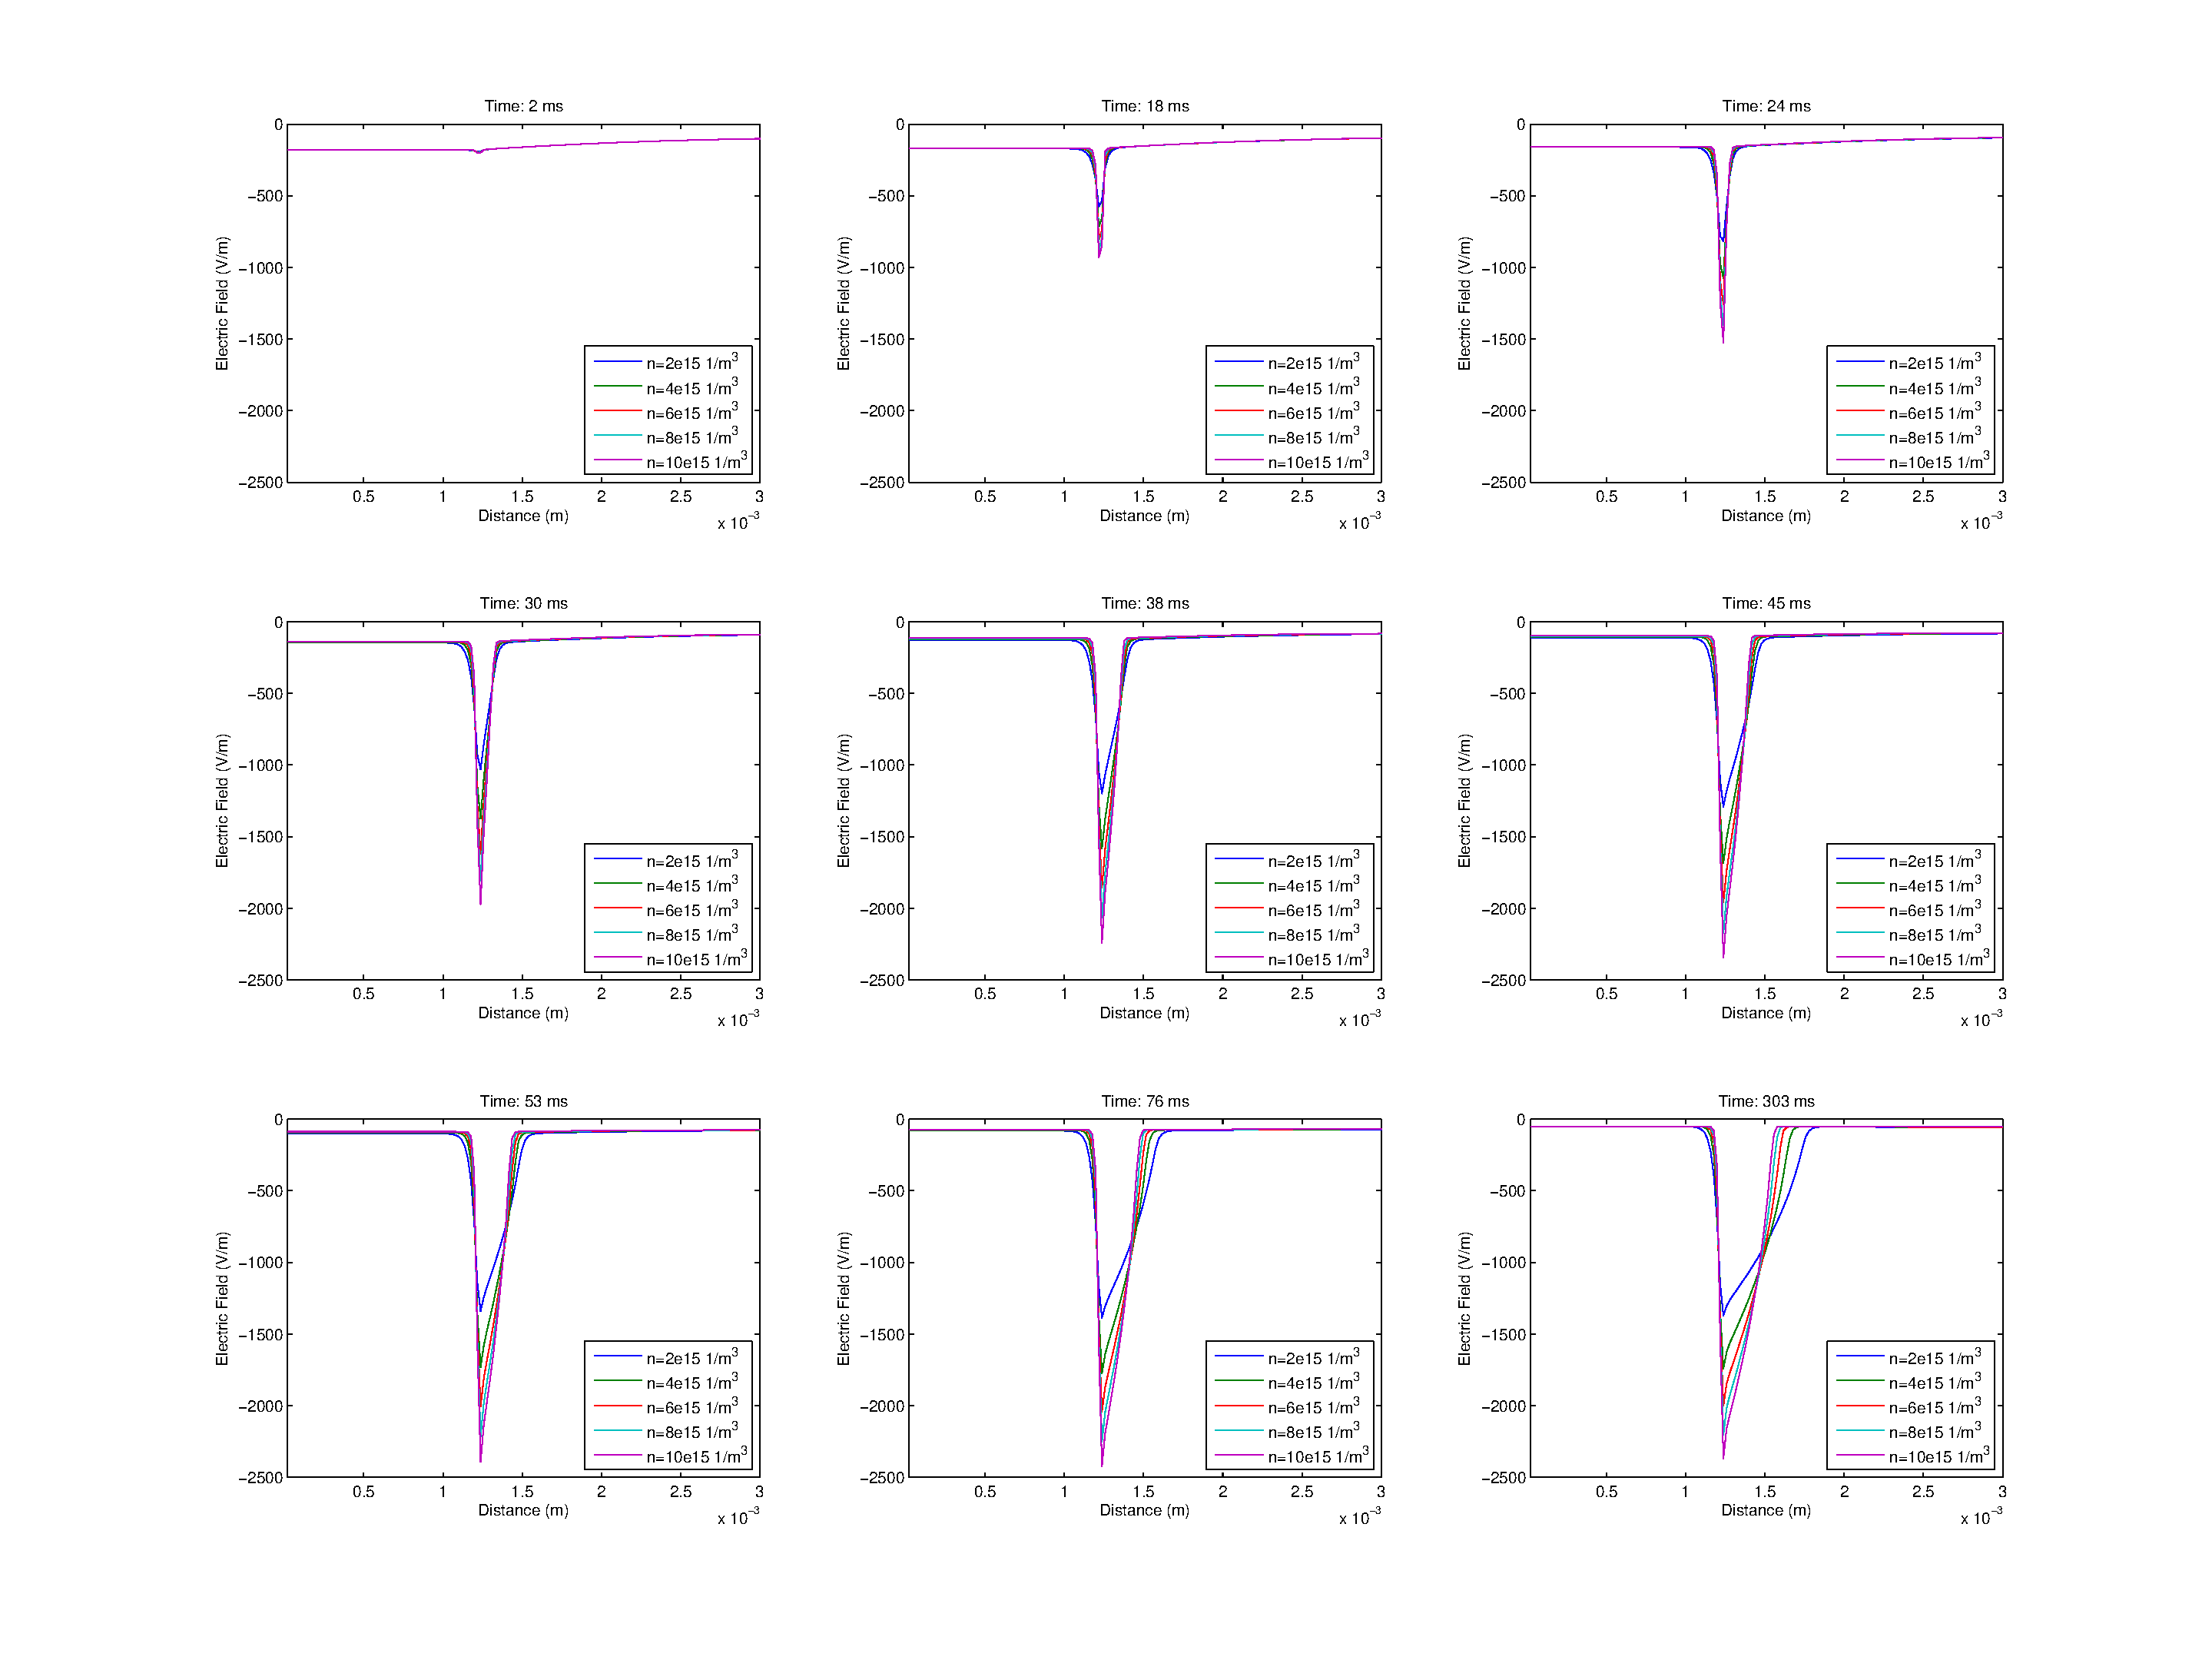
\includegraphics[scale=0.40]{Ex5E_Time1}
\caption{Electric field distribution over time (Note:Not aligned with potential distribution for better visuals) } 
\label{MemE}
\end{figure}
\end{landscape}


\begin{landscape}
\begin{figure}[!htp]
\centering
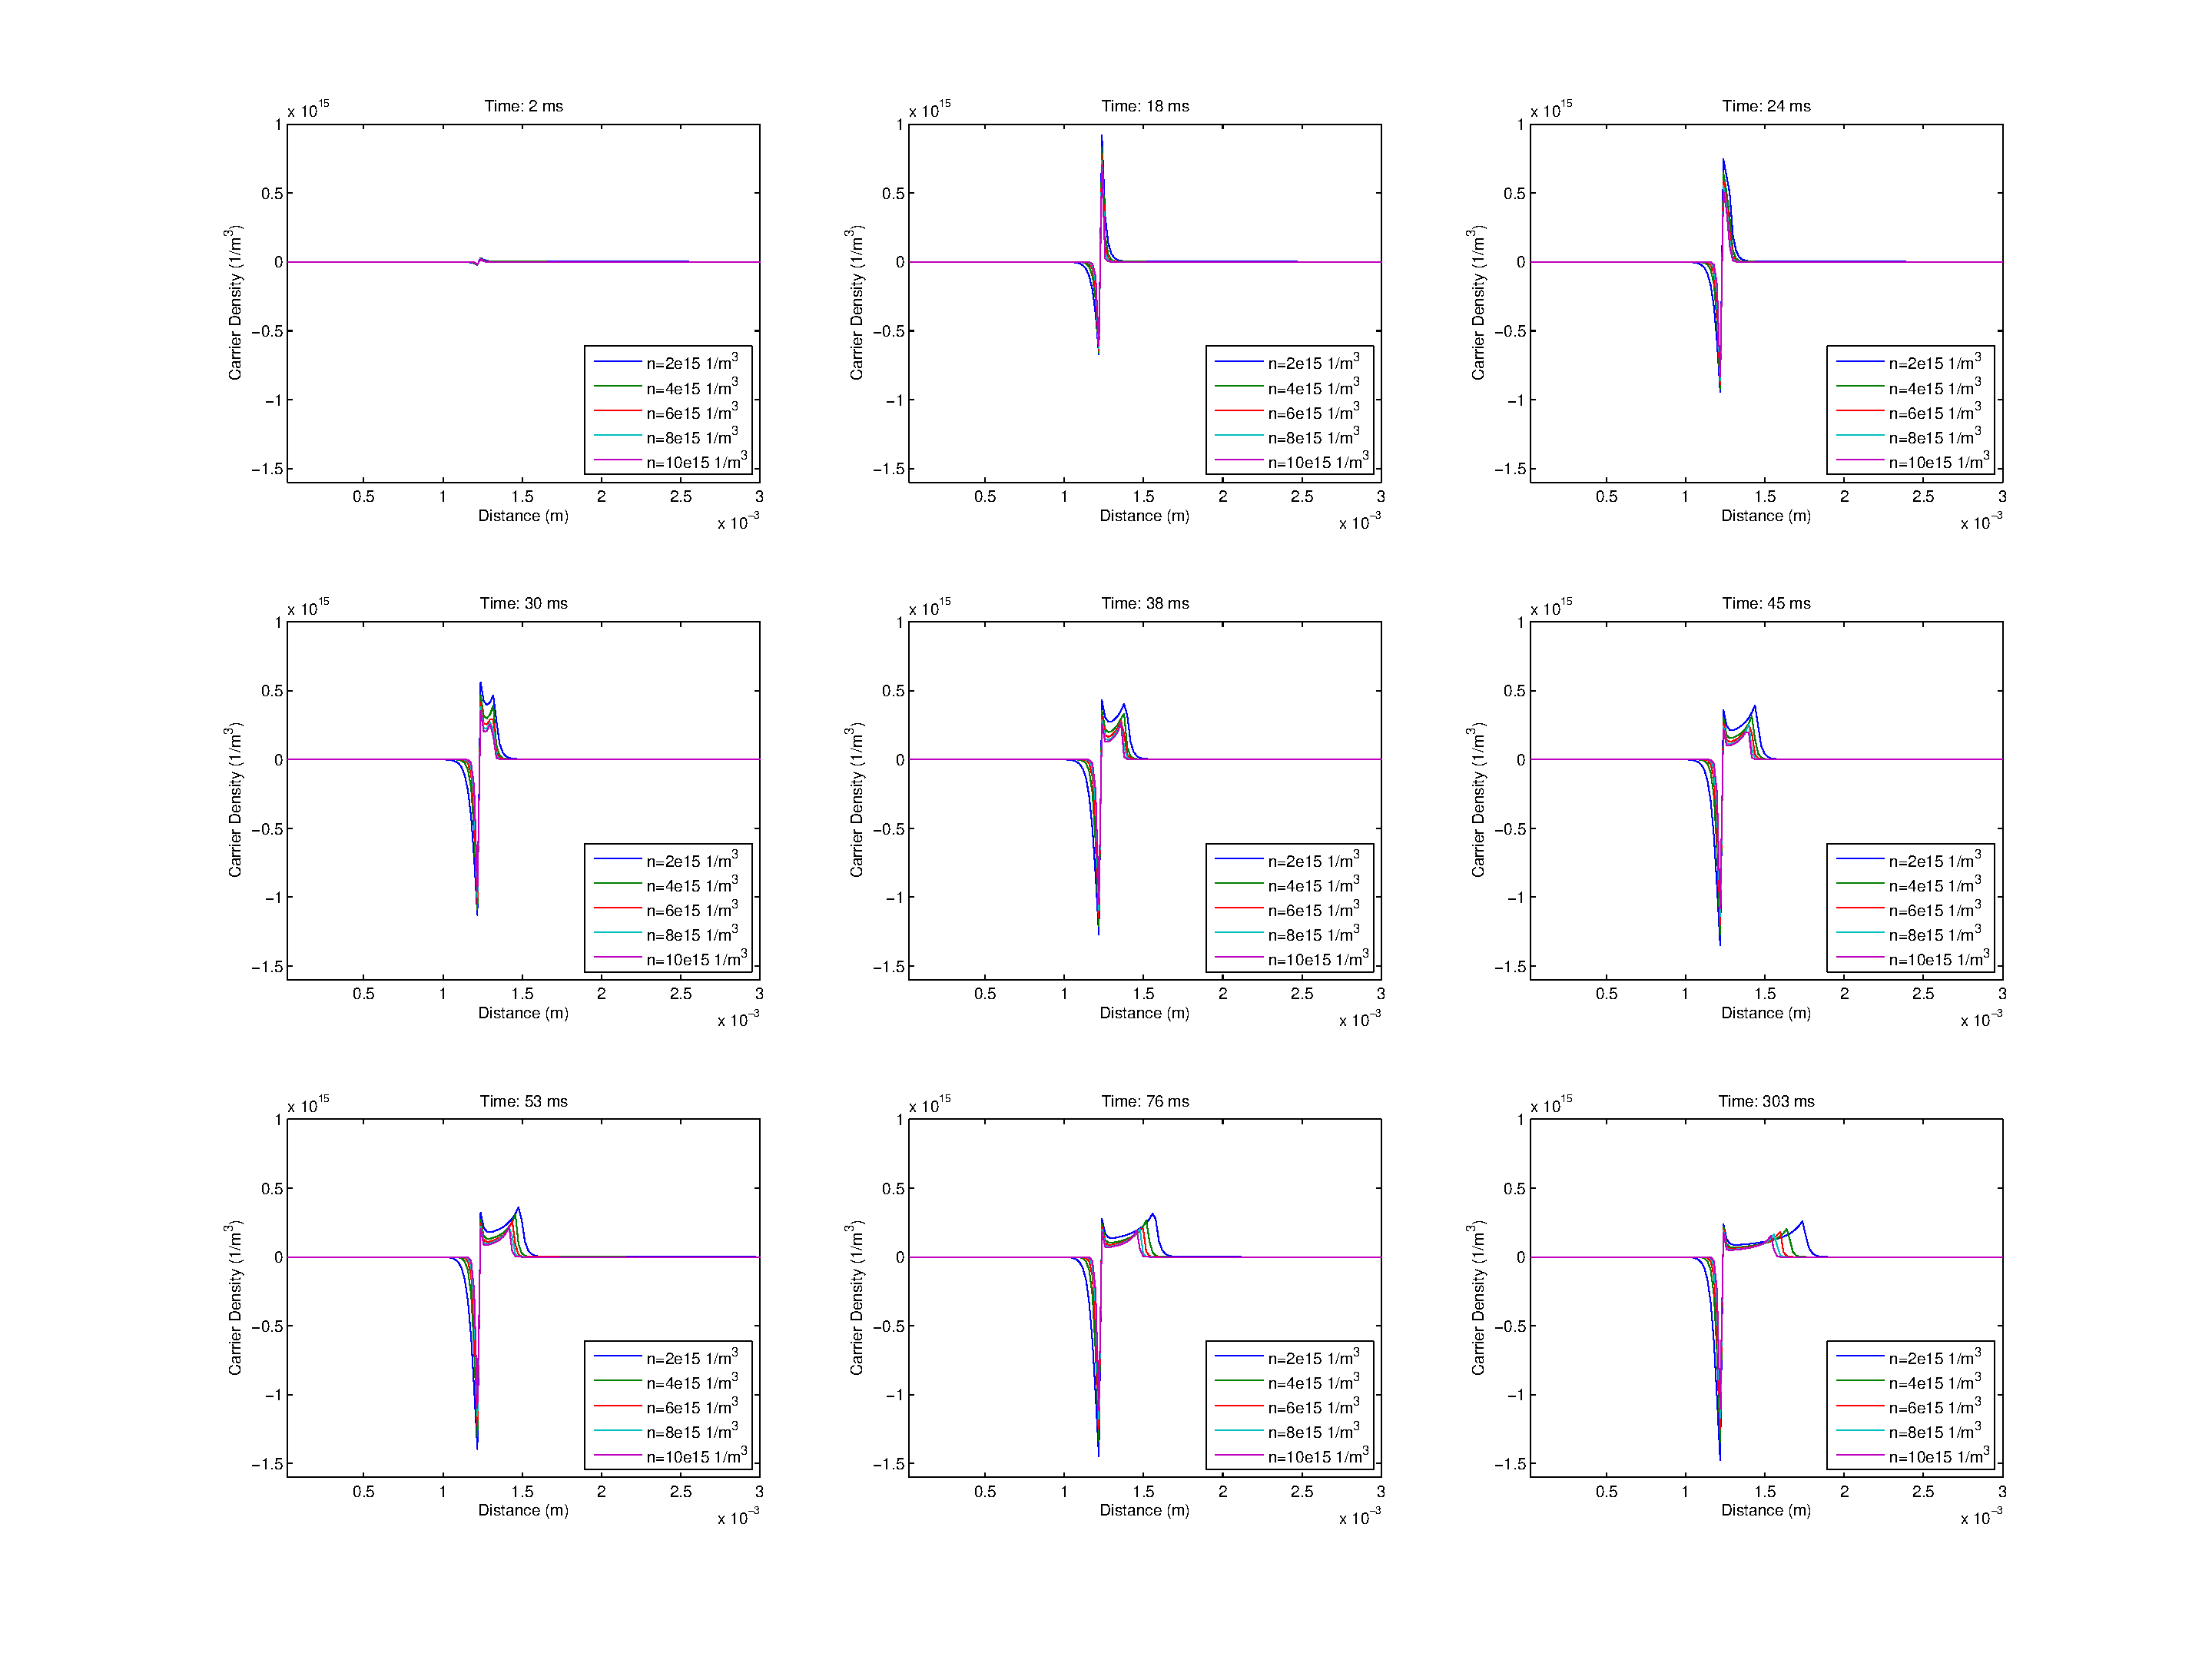
\includegraphics[scale=0.40]{Ex5NetQ_Time1}
\caption{Normalized net charge density distribution over time (Note:Not aligned with potential distribution for better visuals) } 
\label{}
\end{figure}
\end{landscape}


\begin{landscape}
\begin{figure}[!htp]
\centering
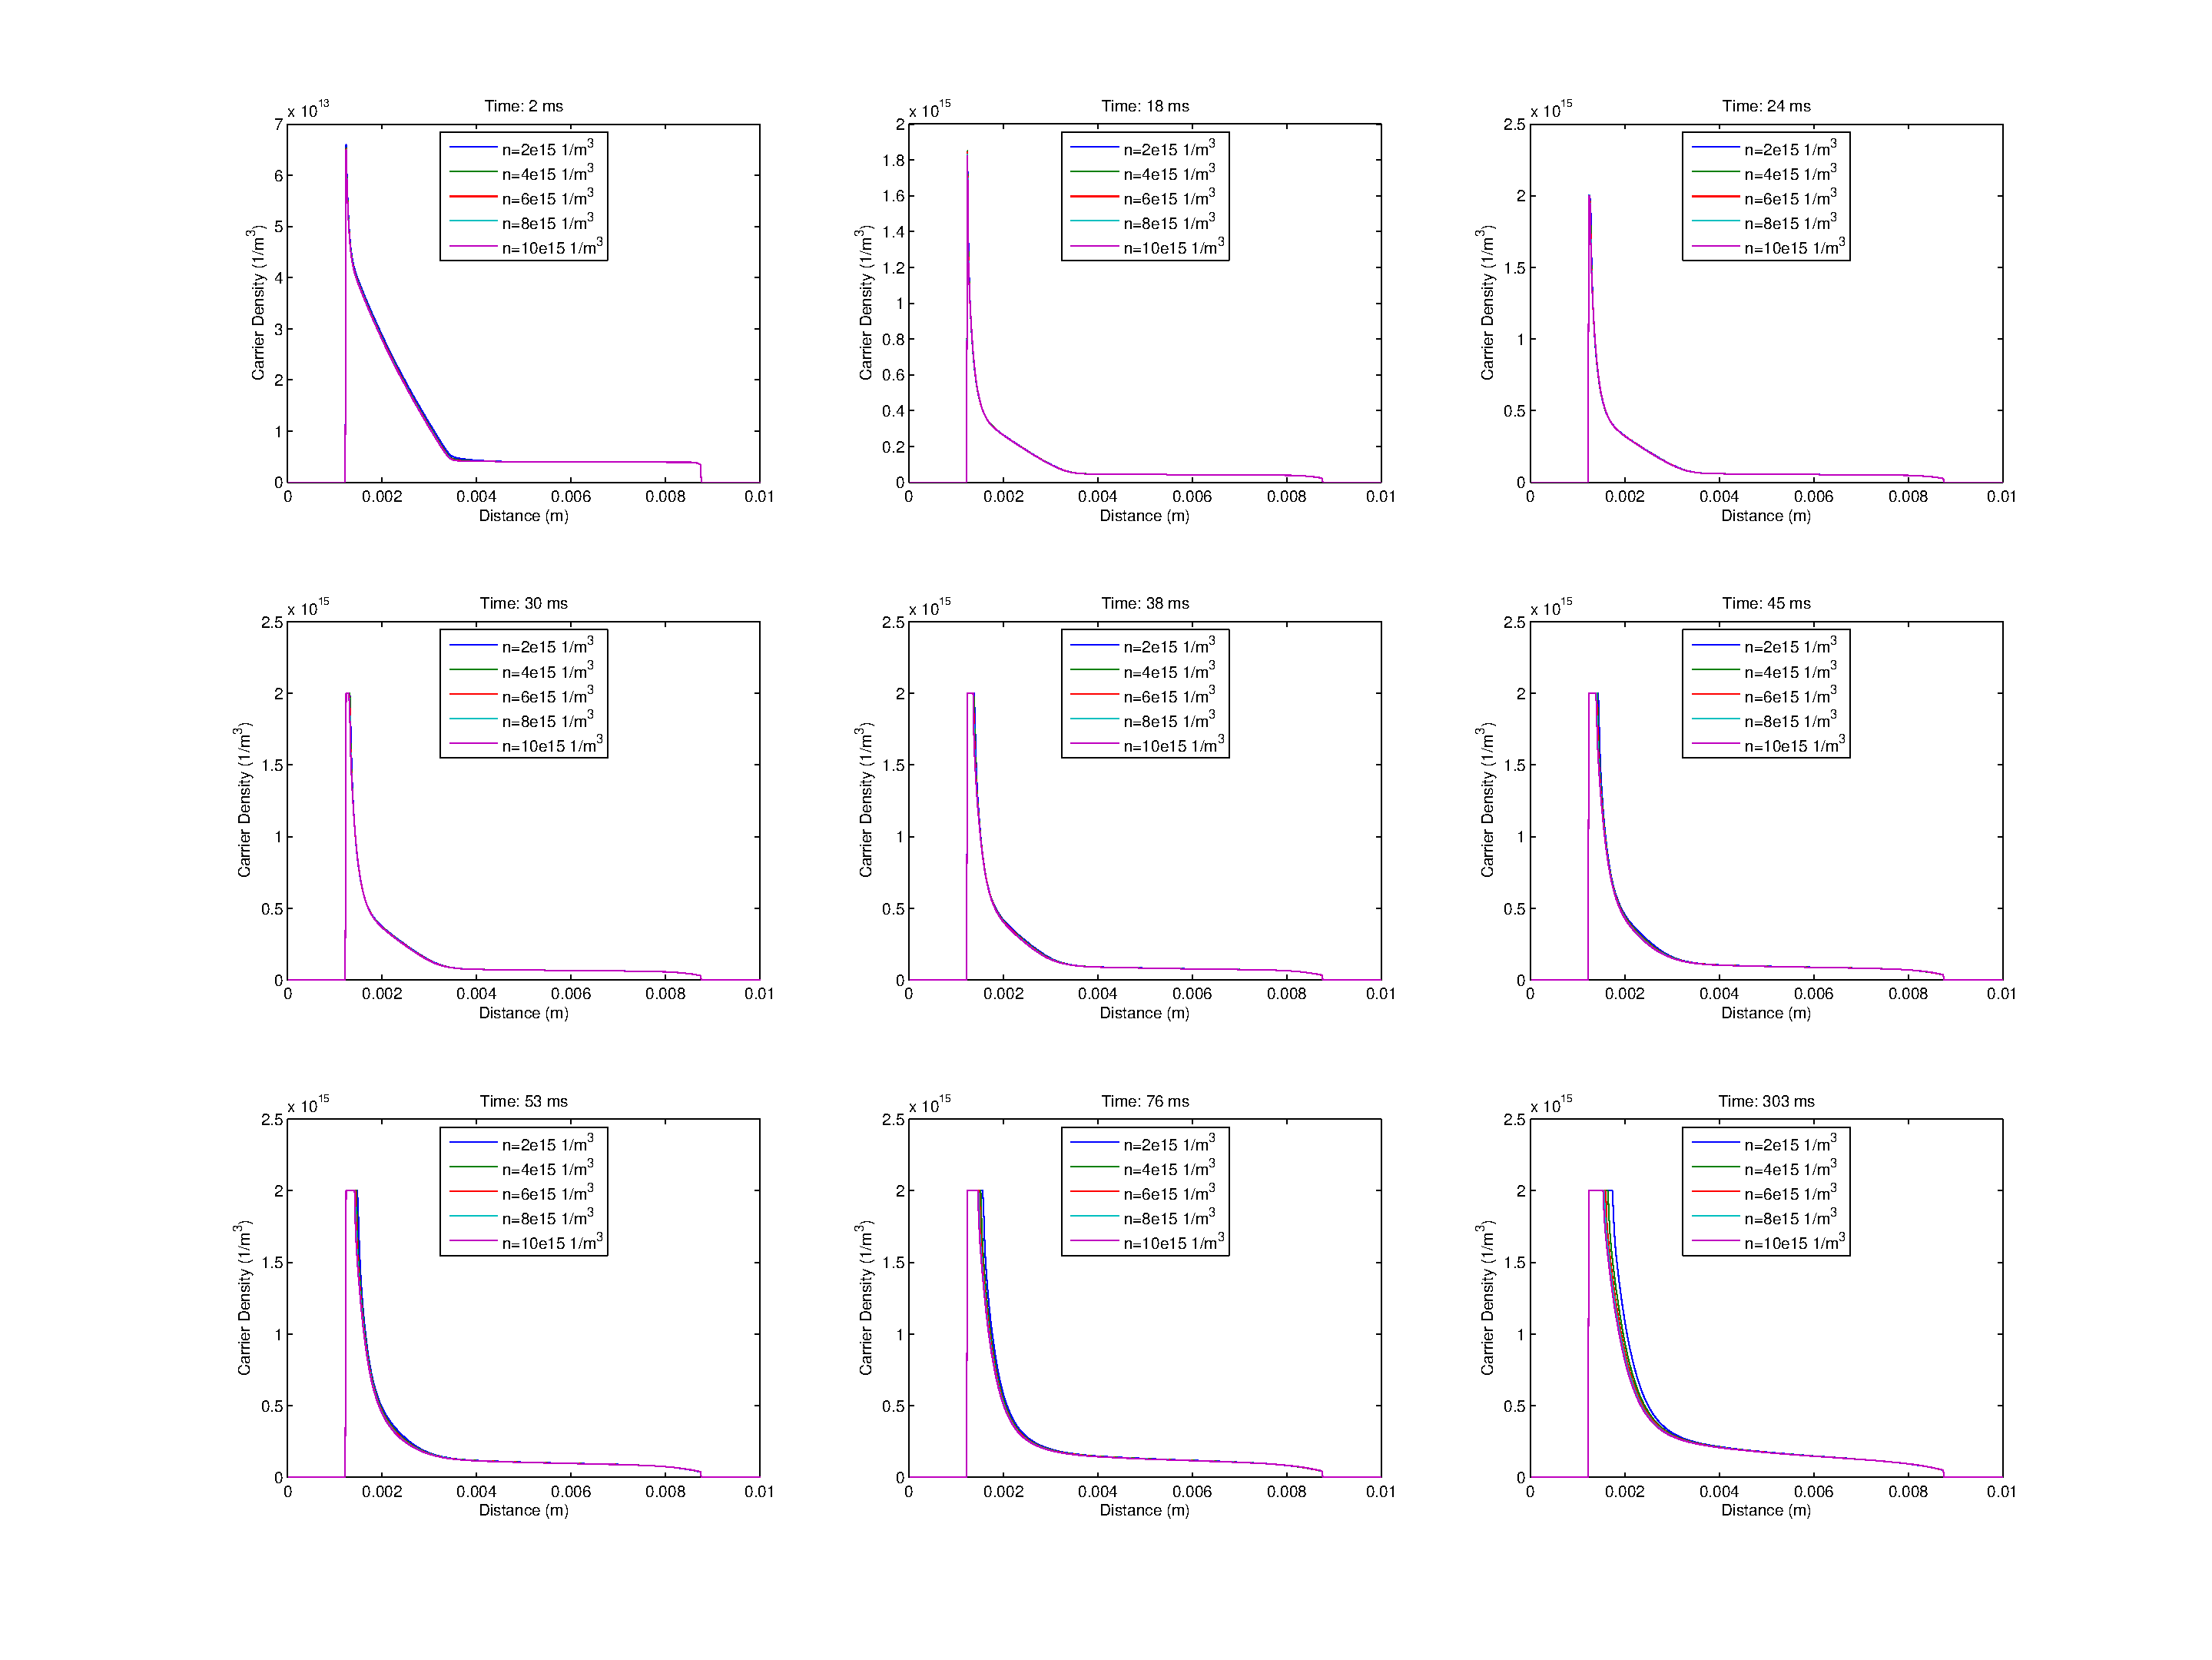
\includegraphics[scale=0.40]{Ex5Np_Time1}
\caption{Normalized lithium density distribution over time} 
\label{}
\end{figure}
\end{landscape}


\begin{landscape}
\begin{figure}[!htp]
\centering
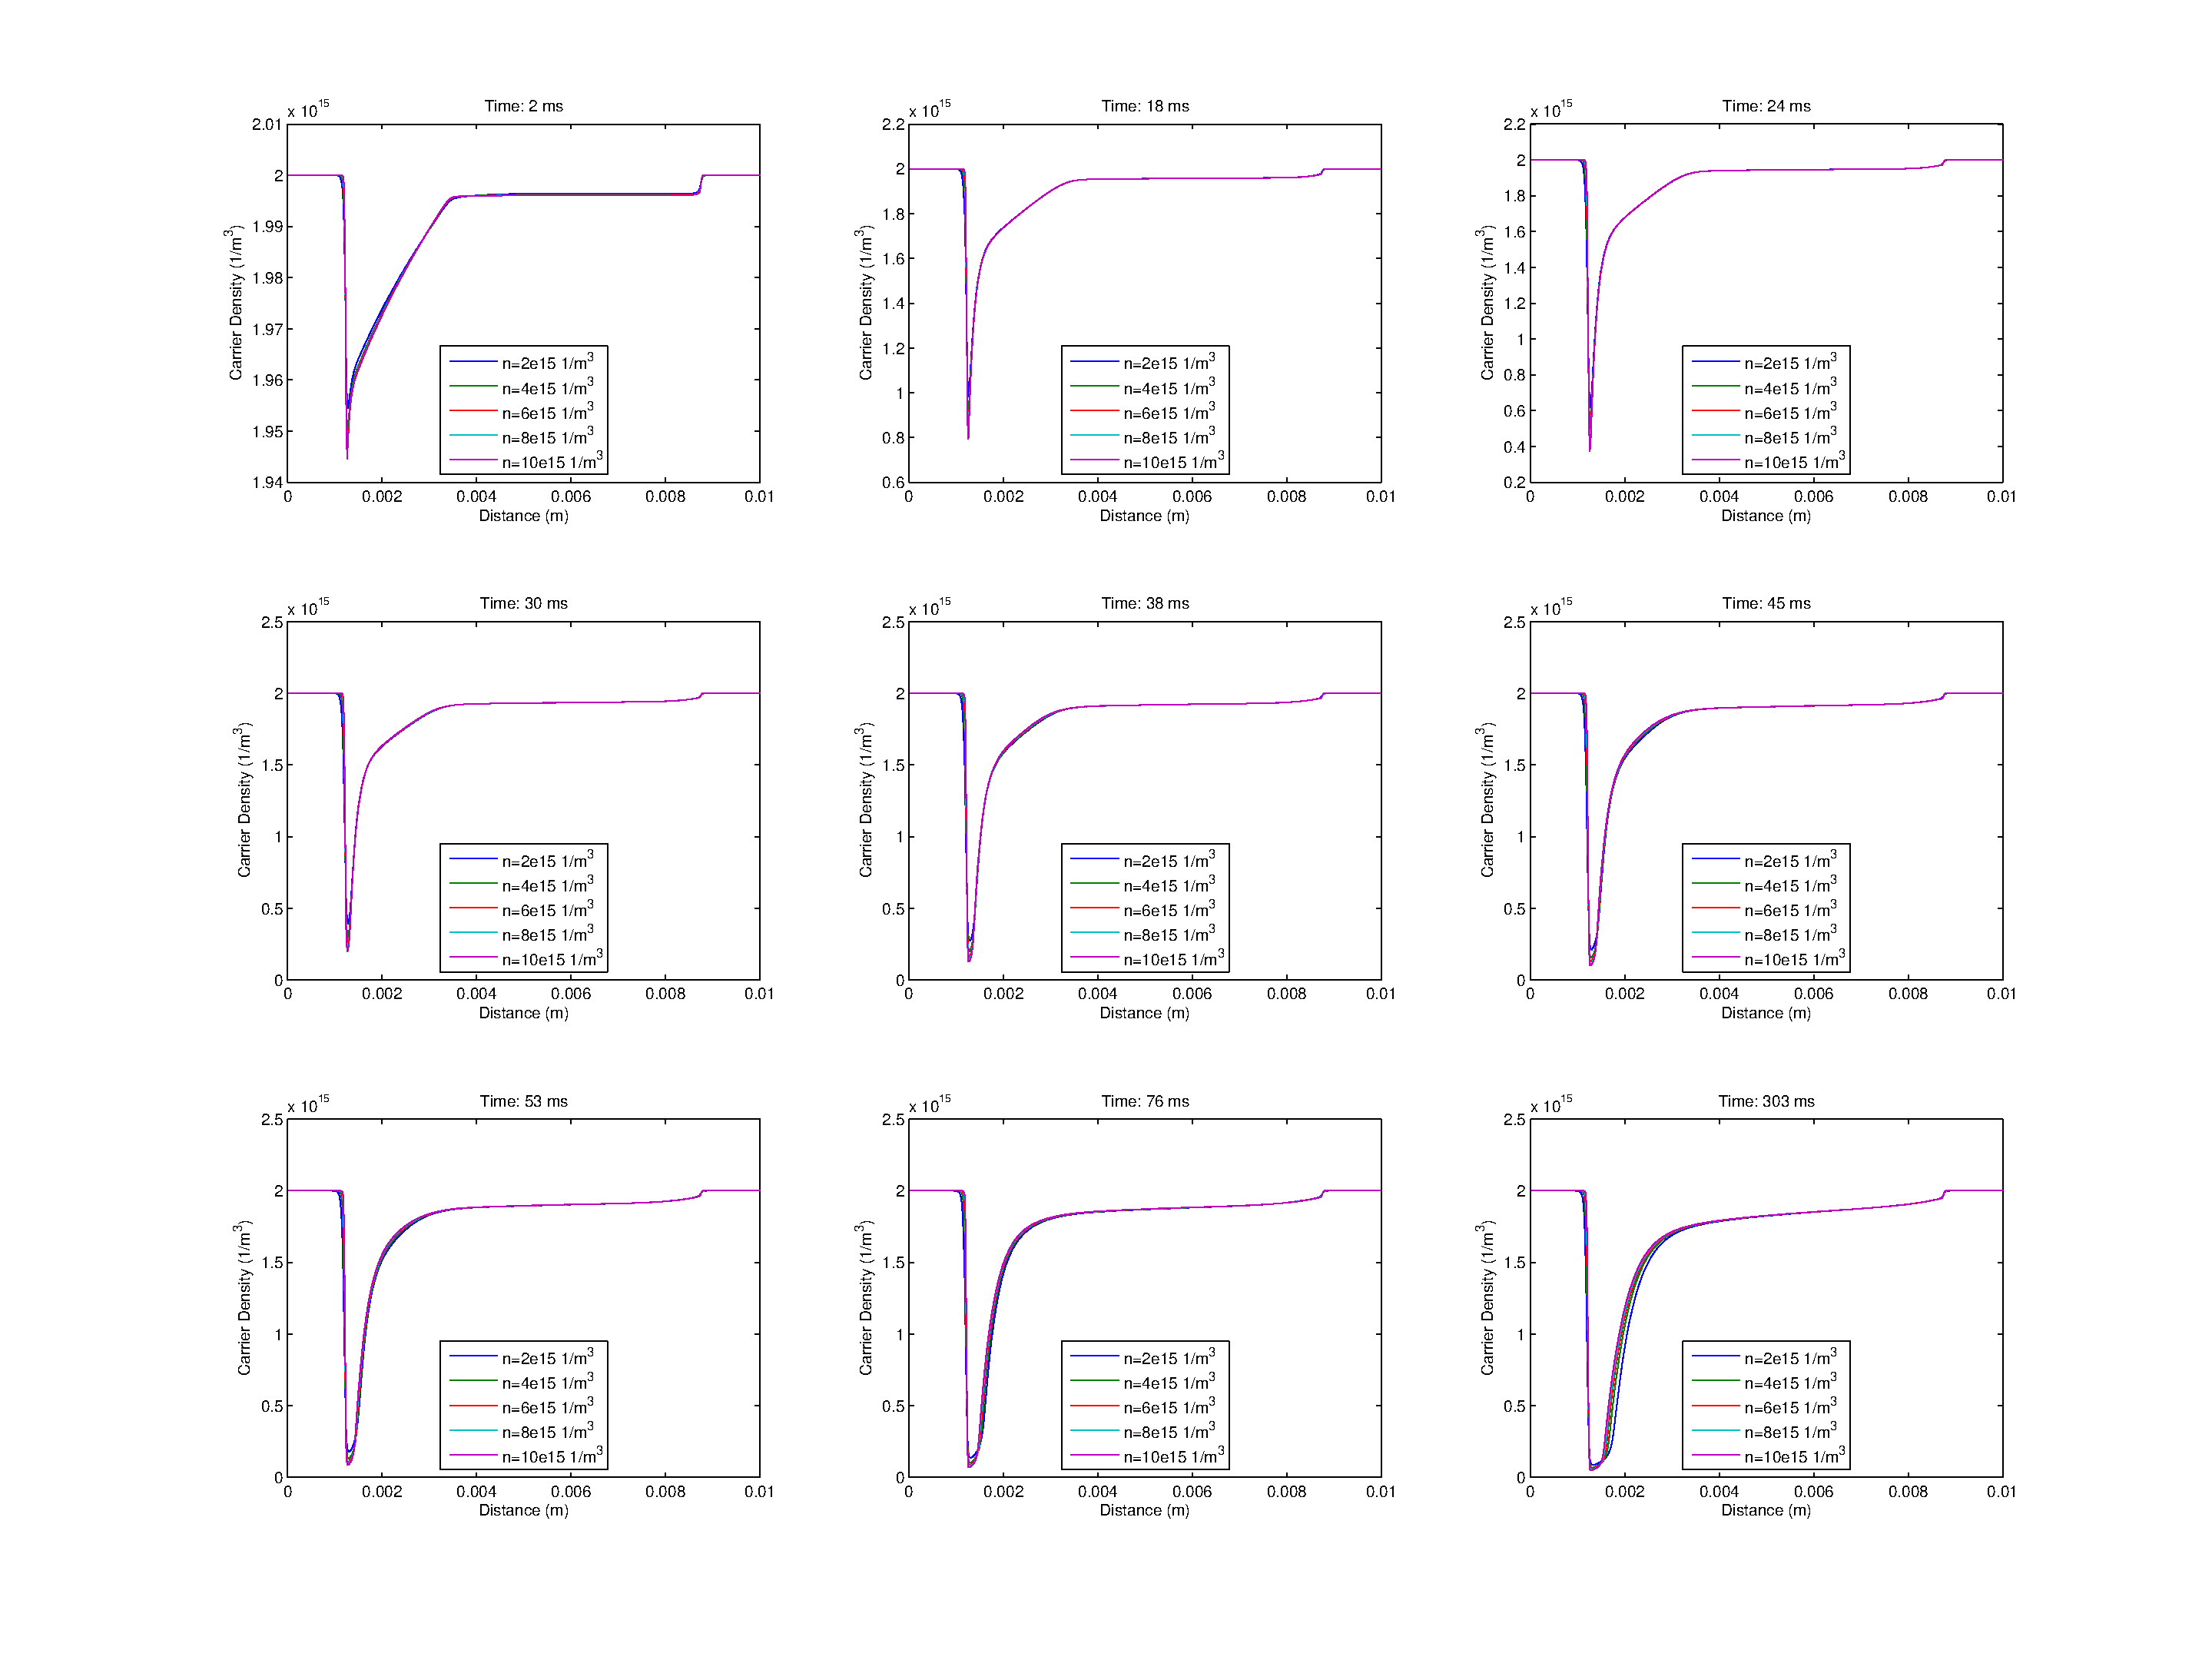
\includegraphics[scale=0.40]{Ex5p_Time1}
\caption{Normalized hole density distribution over time} 
\label{}
\end{figure}
\end{landscape}

\section{1-D Memristor with Notch (Cross section 2)}
\begin{landscape}
\begin{figure}[!htp]
\centering
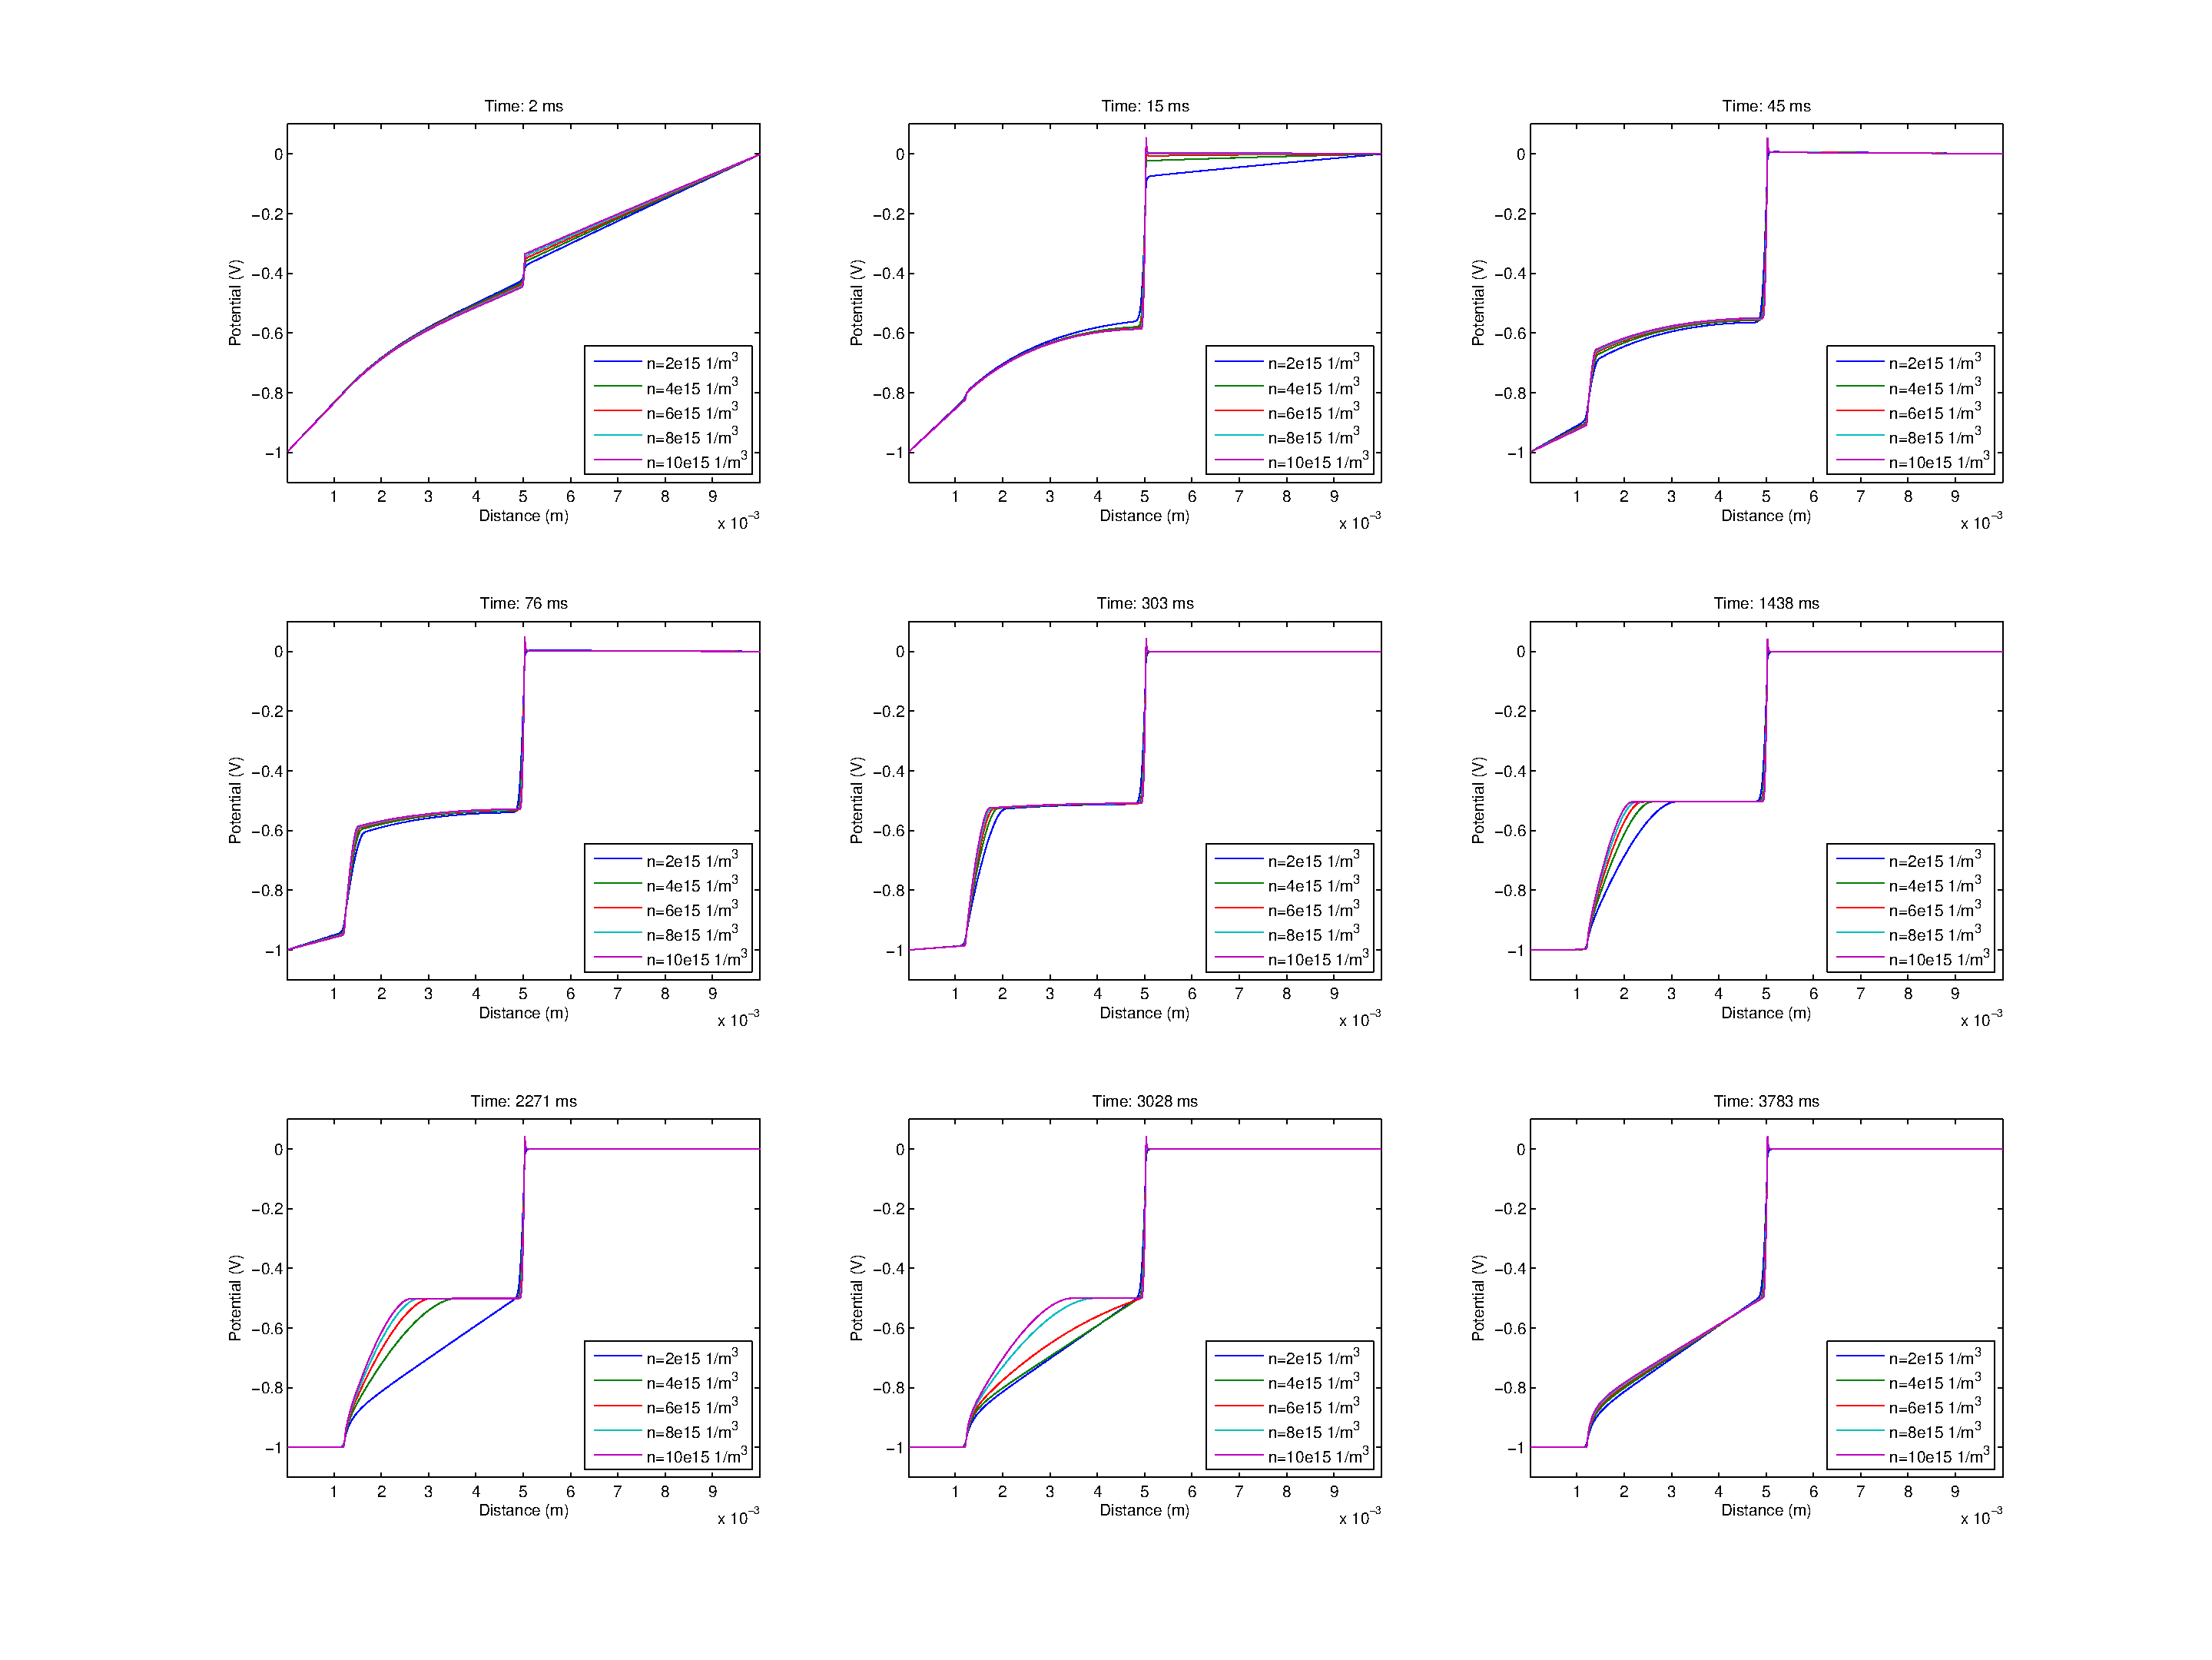
\includegraphics[scale=0.40]{Ex5V_Notch_Time1}
\caption{Notched memristor potential distribution over time} 
\label{}
\end{figure}
\end{landscape}

\begin{landscape}
\begin{figure}[!htp]
\centering
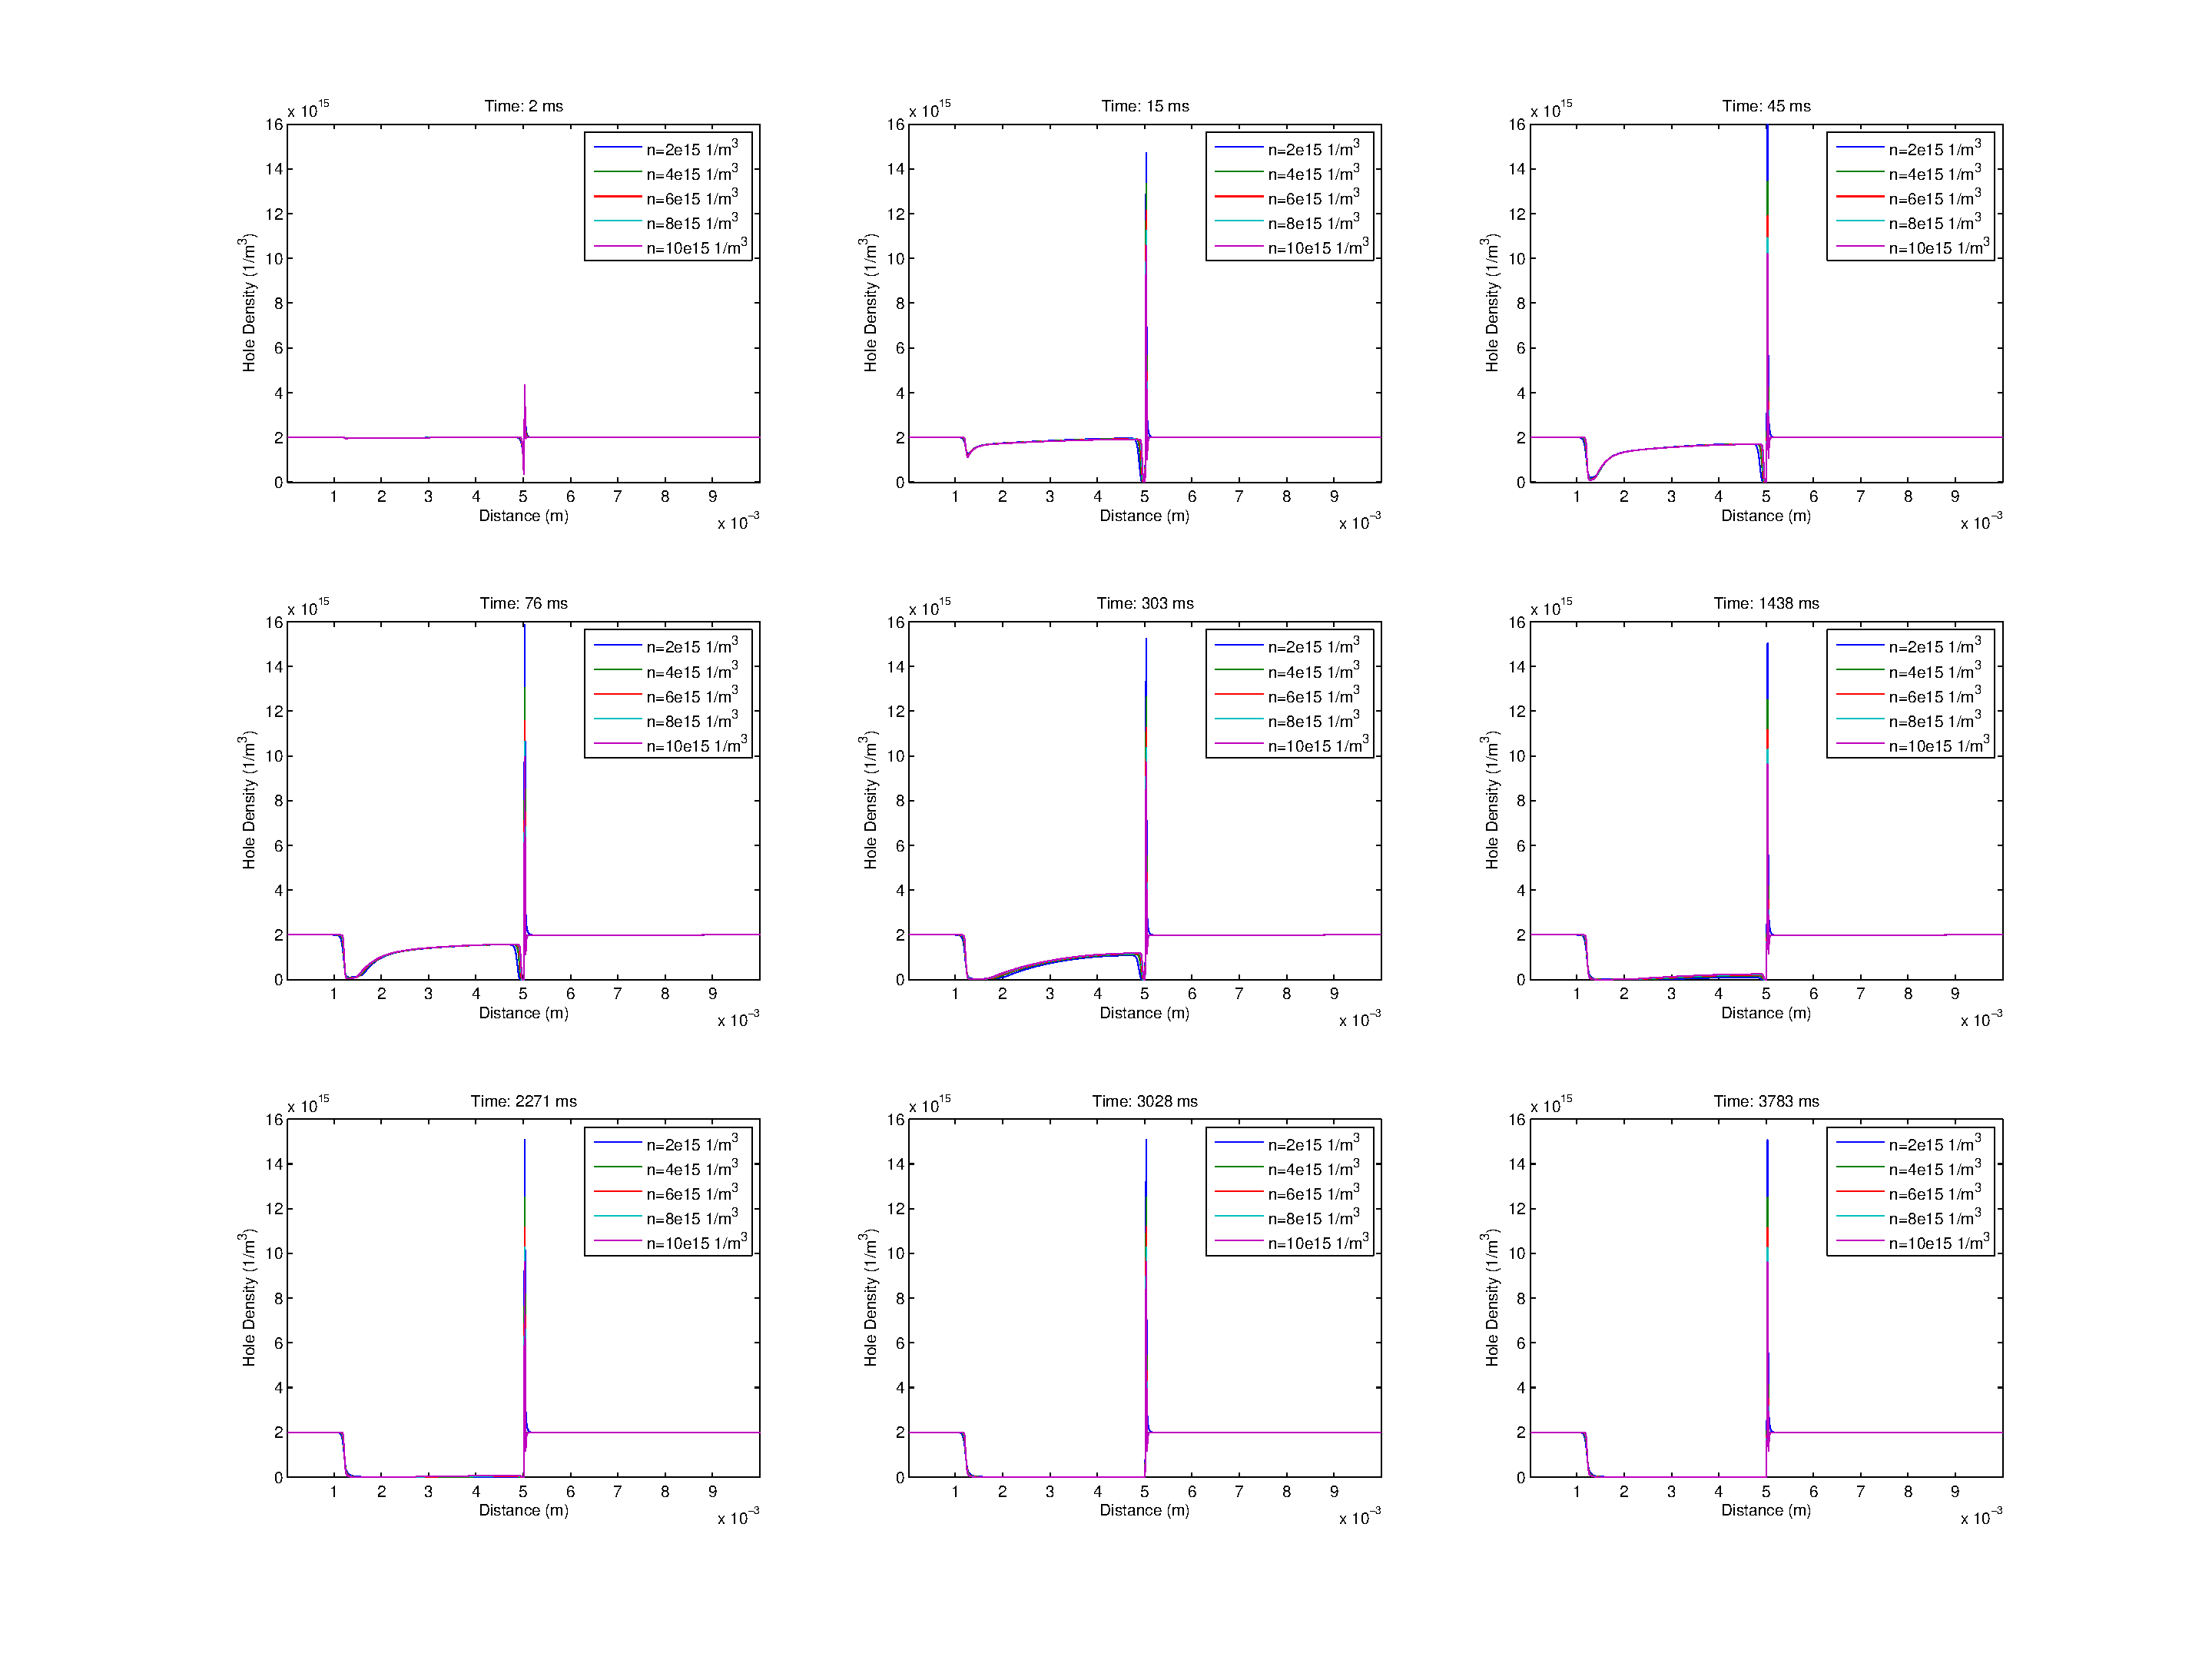
\includegraphics[scale=0.40]{Ex5Hole_Notch_Time1}
\caption{Normalized hole distribution over time} 
\label{}
\end{figure}
\end{landscape}


\begin{landscape}
\begin{figure}[!htp]
\centering
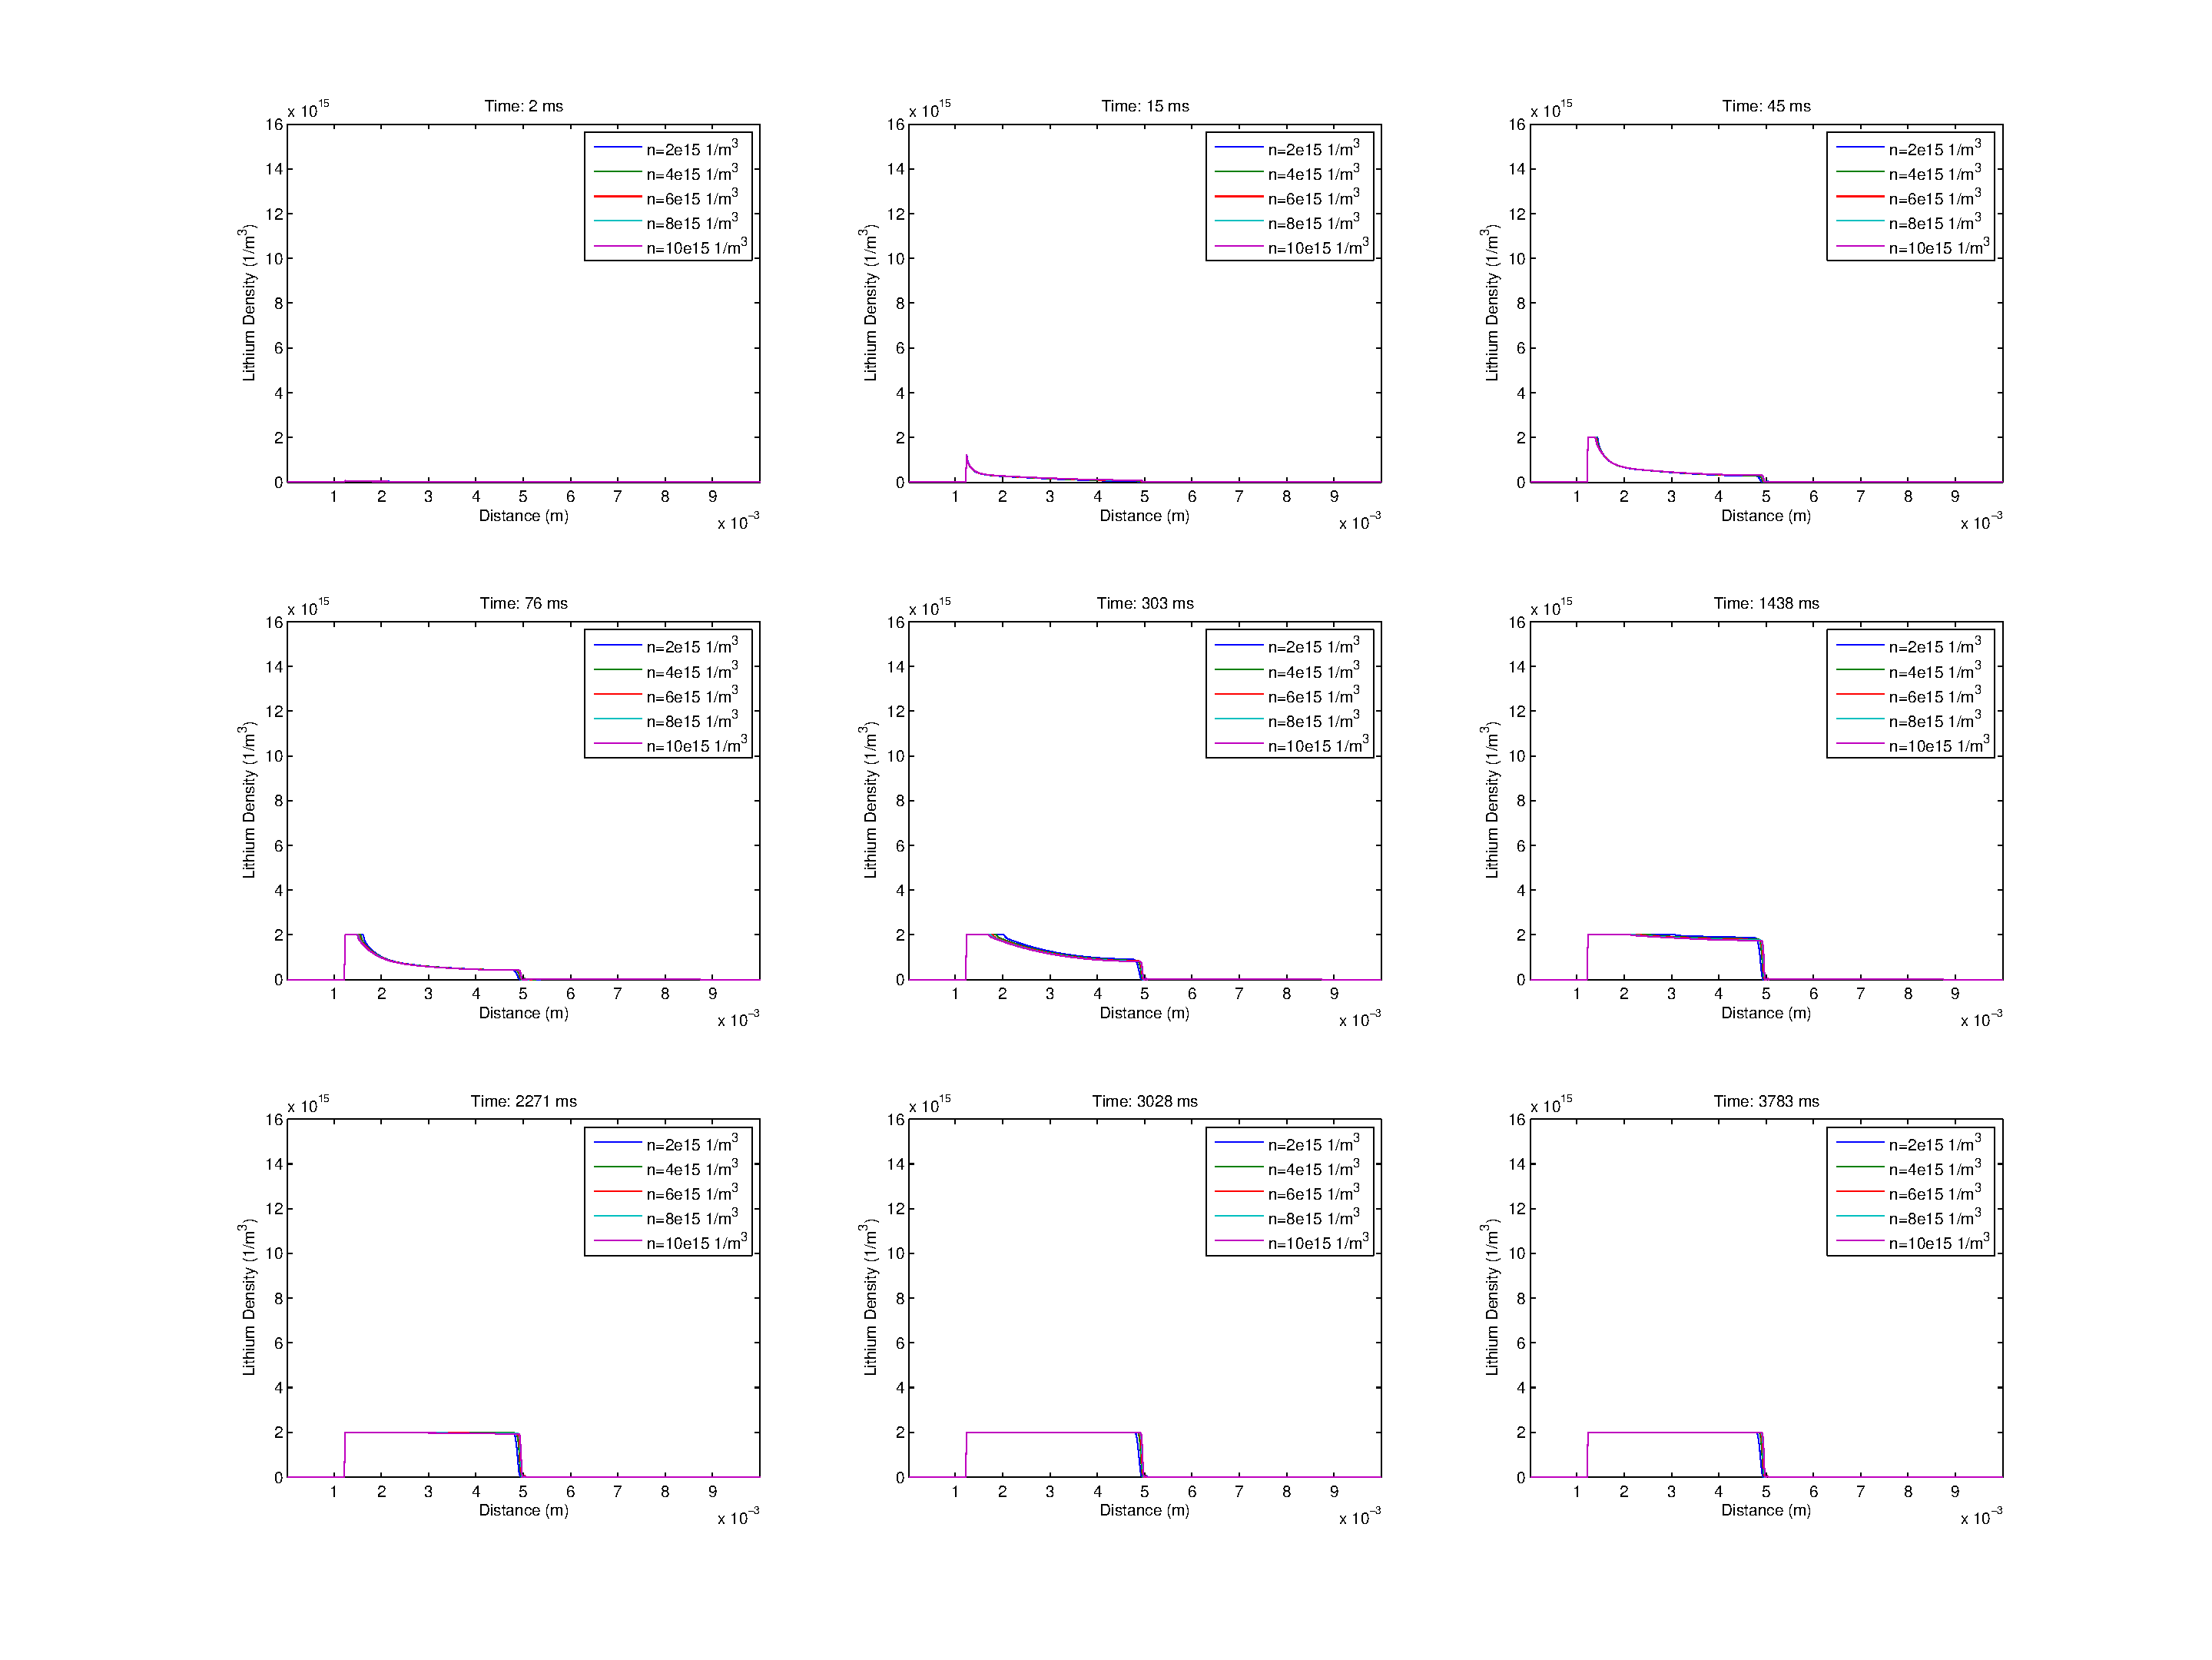
\includegraphics[scale=0.40]{Ex5Li_Notch_Time1}
\caption{Normalized lithium distribution over time} 
\label{}
\end{figure}
\end{landscape}


\begin{landscape}
\begin{figure}[!htp]
\centering
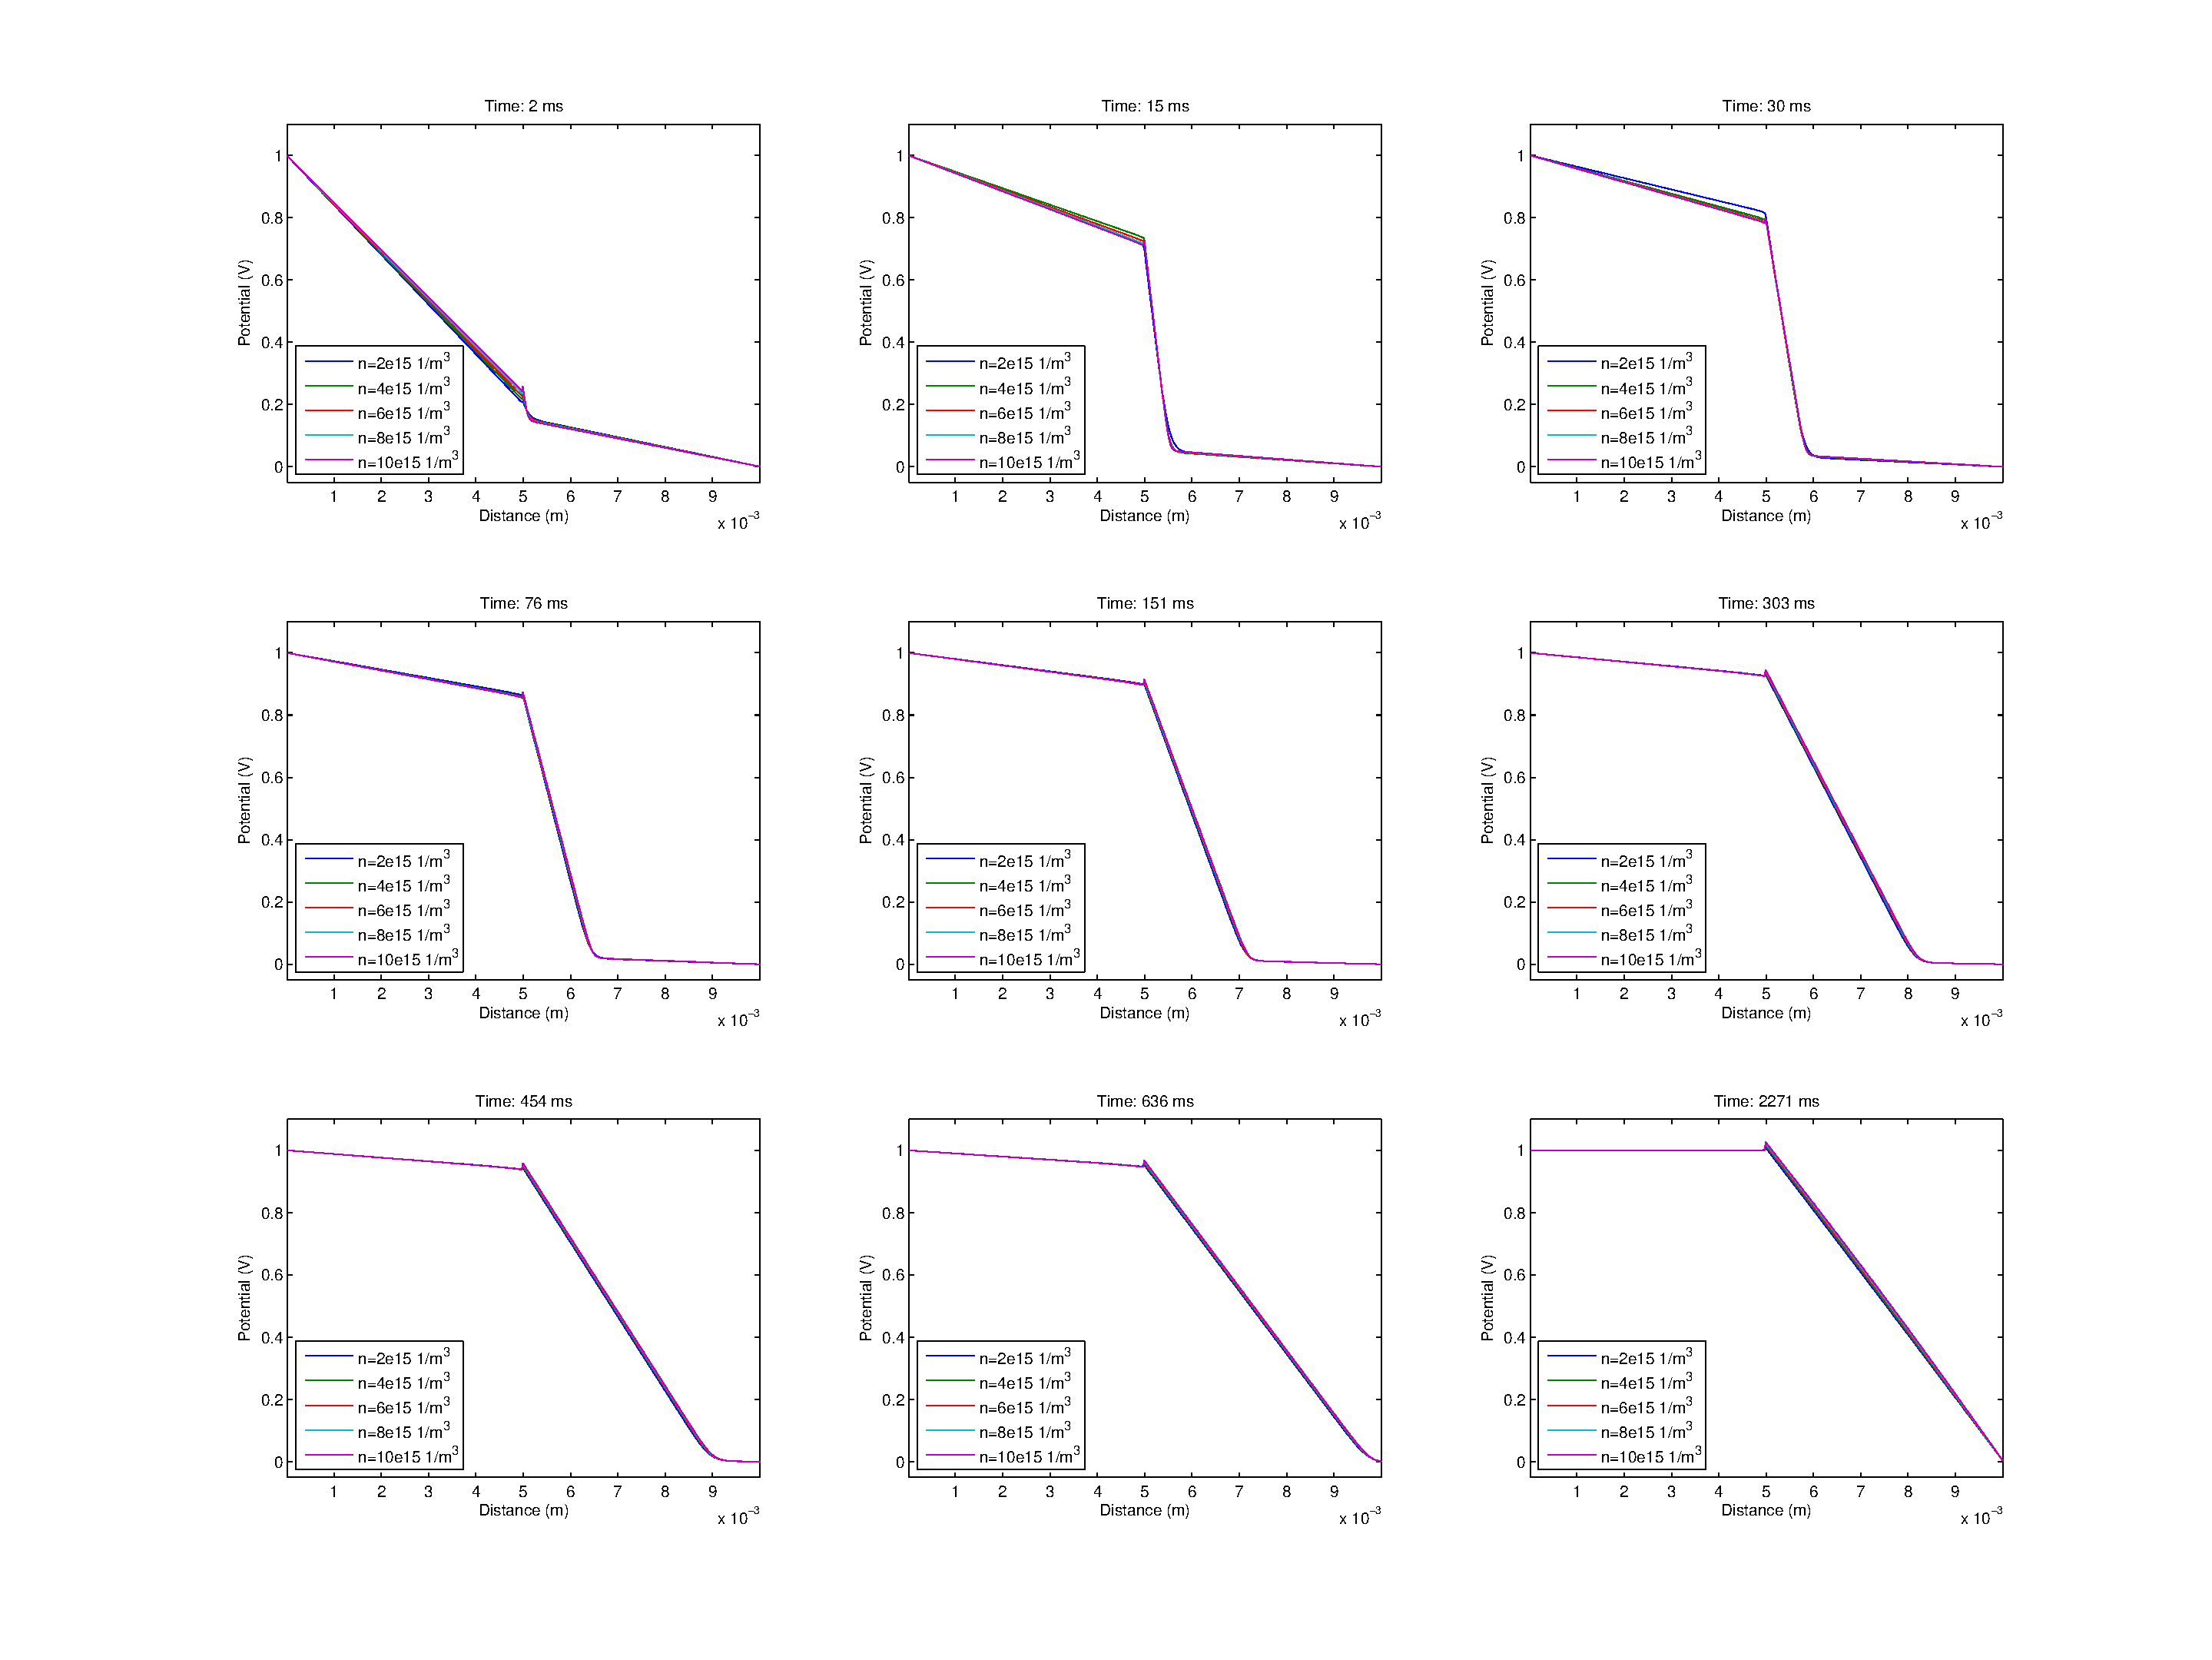
\includegraphics[scale=0.40]{Ex4V_Time}
\caption{Electrolyte/PEDOT interface potential distribution over time} 
\label{}
\end{figure}
\end{landscape}



\section{Electrolyte/PEDOT Interface}
\begin{landscape}
\begin{figure}[!htp]
\centering
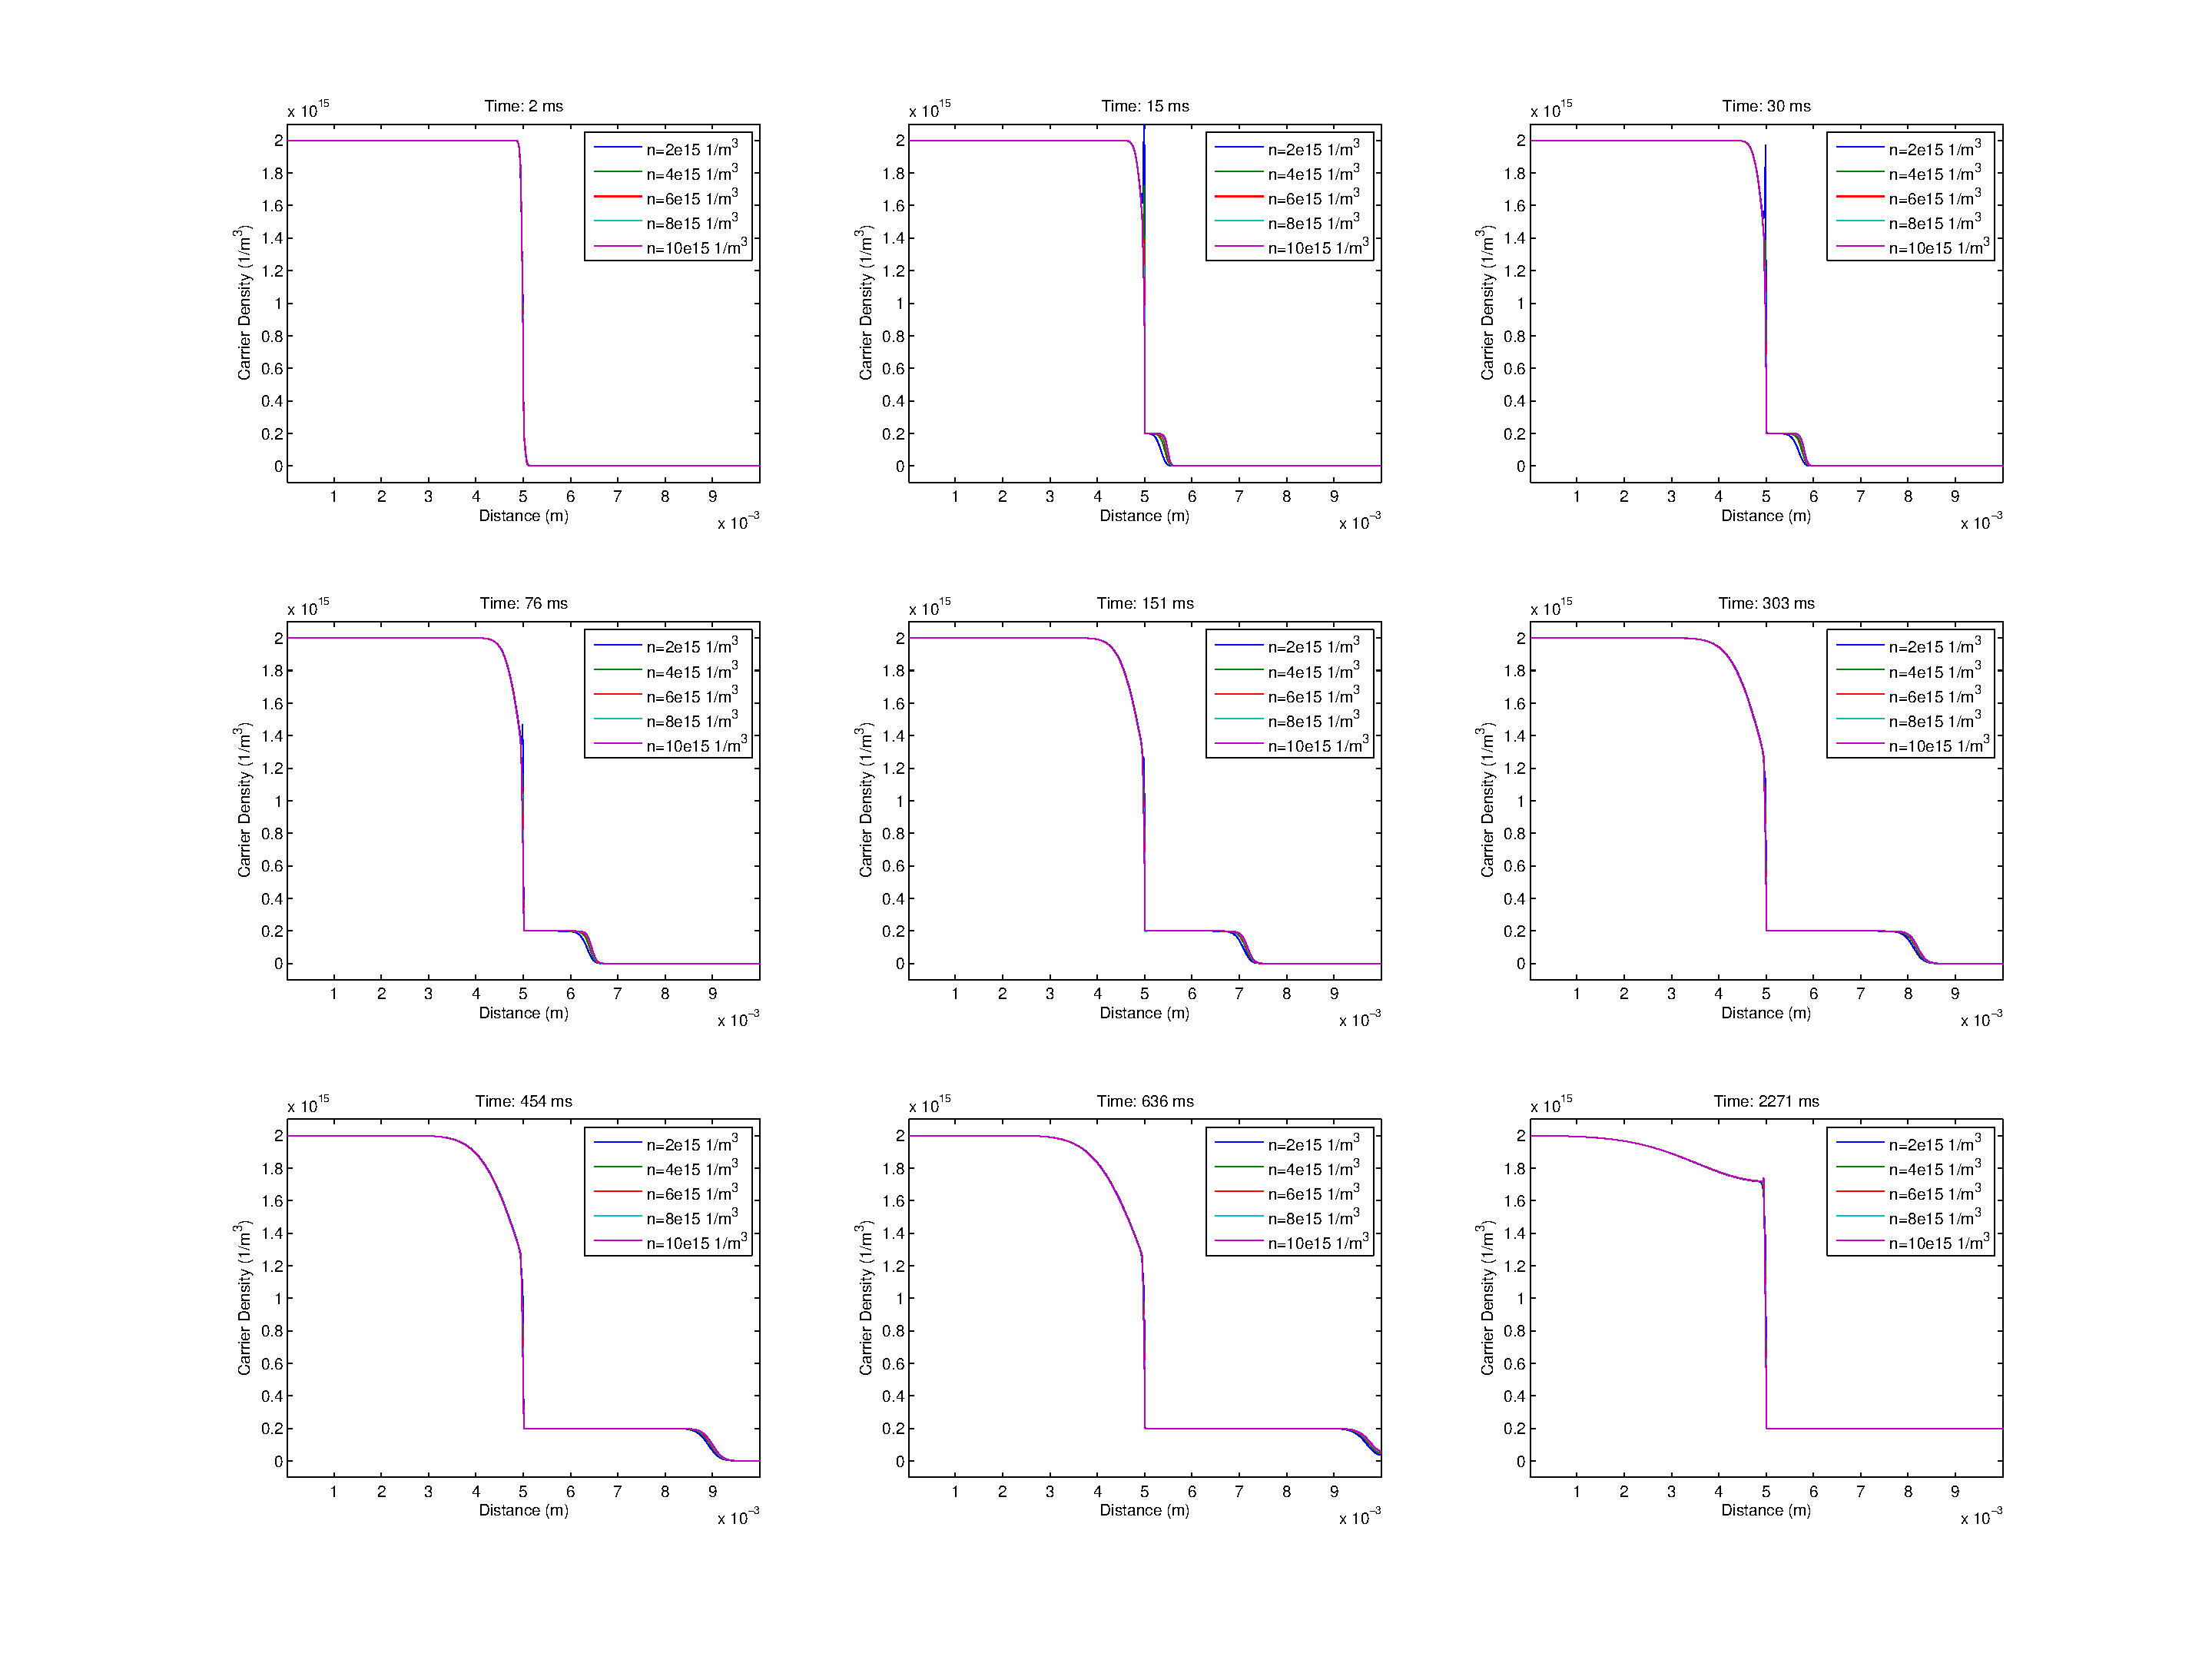
\includegraphics[scale=0.40]{Ex4Np_Time}
\caption{Normalized lithium distribution over time} 
\label{}
\end{figure}
\end{landscape}

\begin{landscape}
\begin{figure}[!htp]
\centering
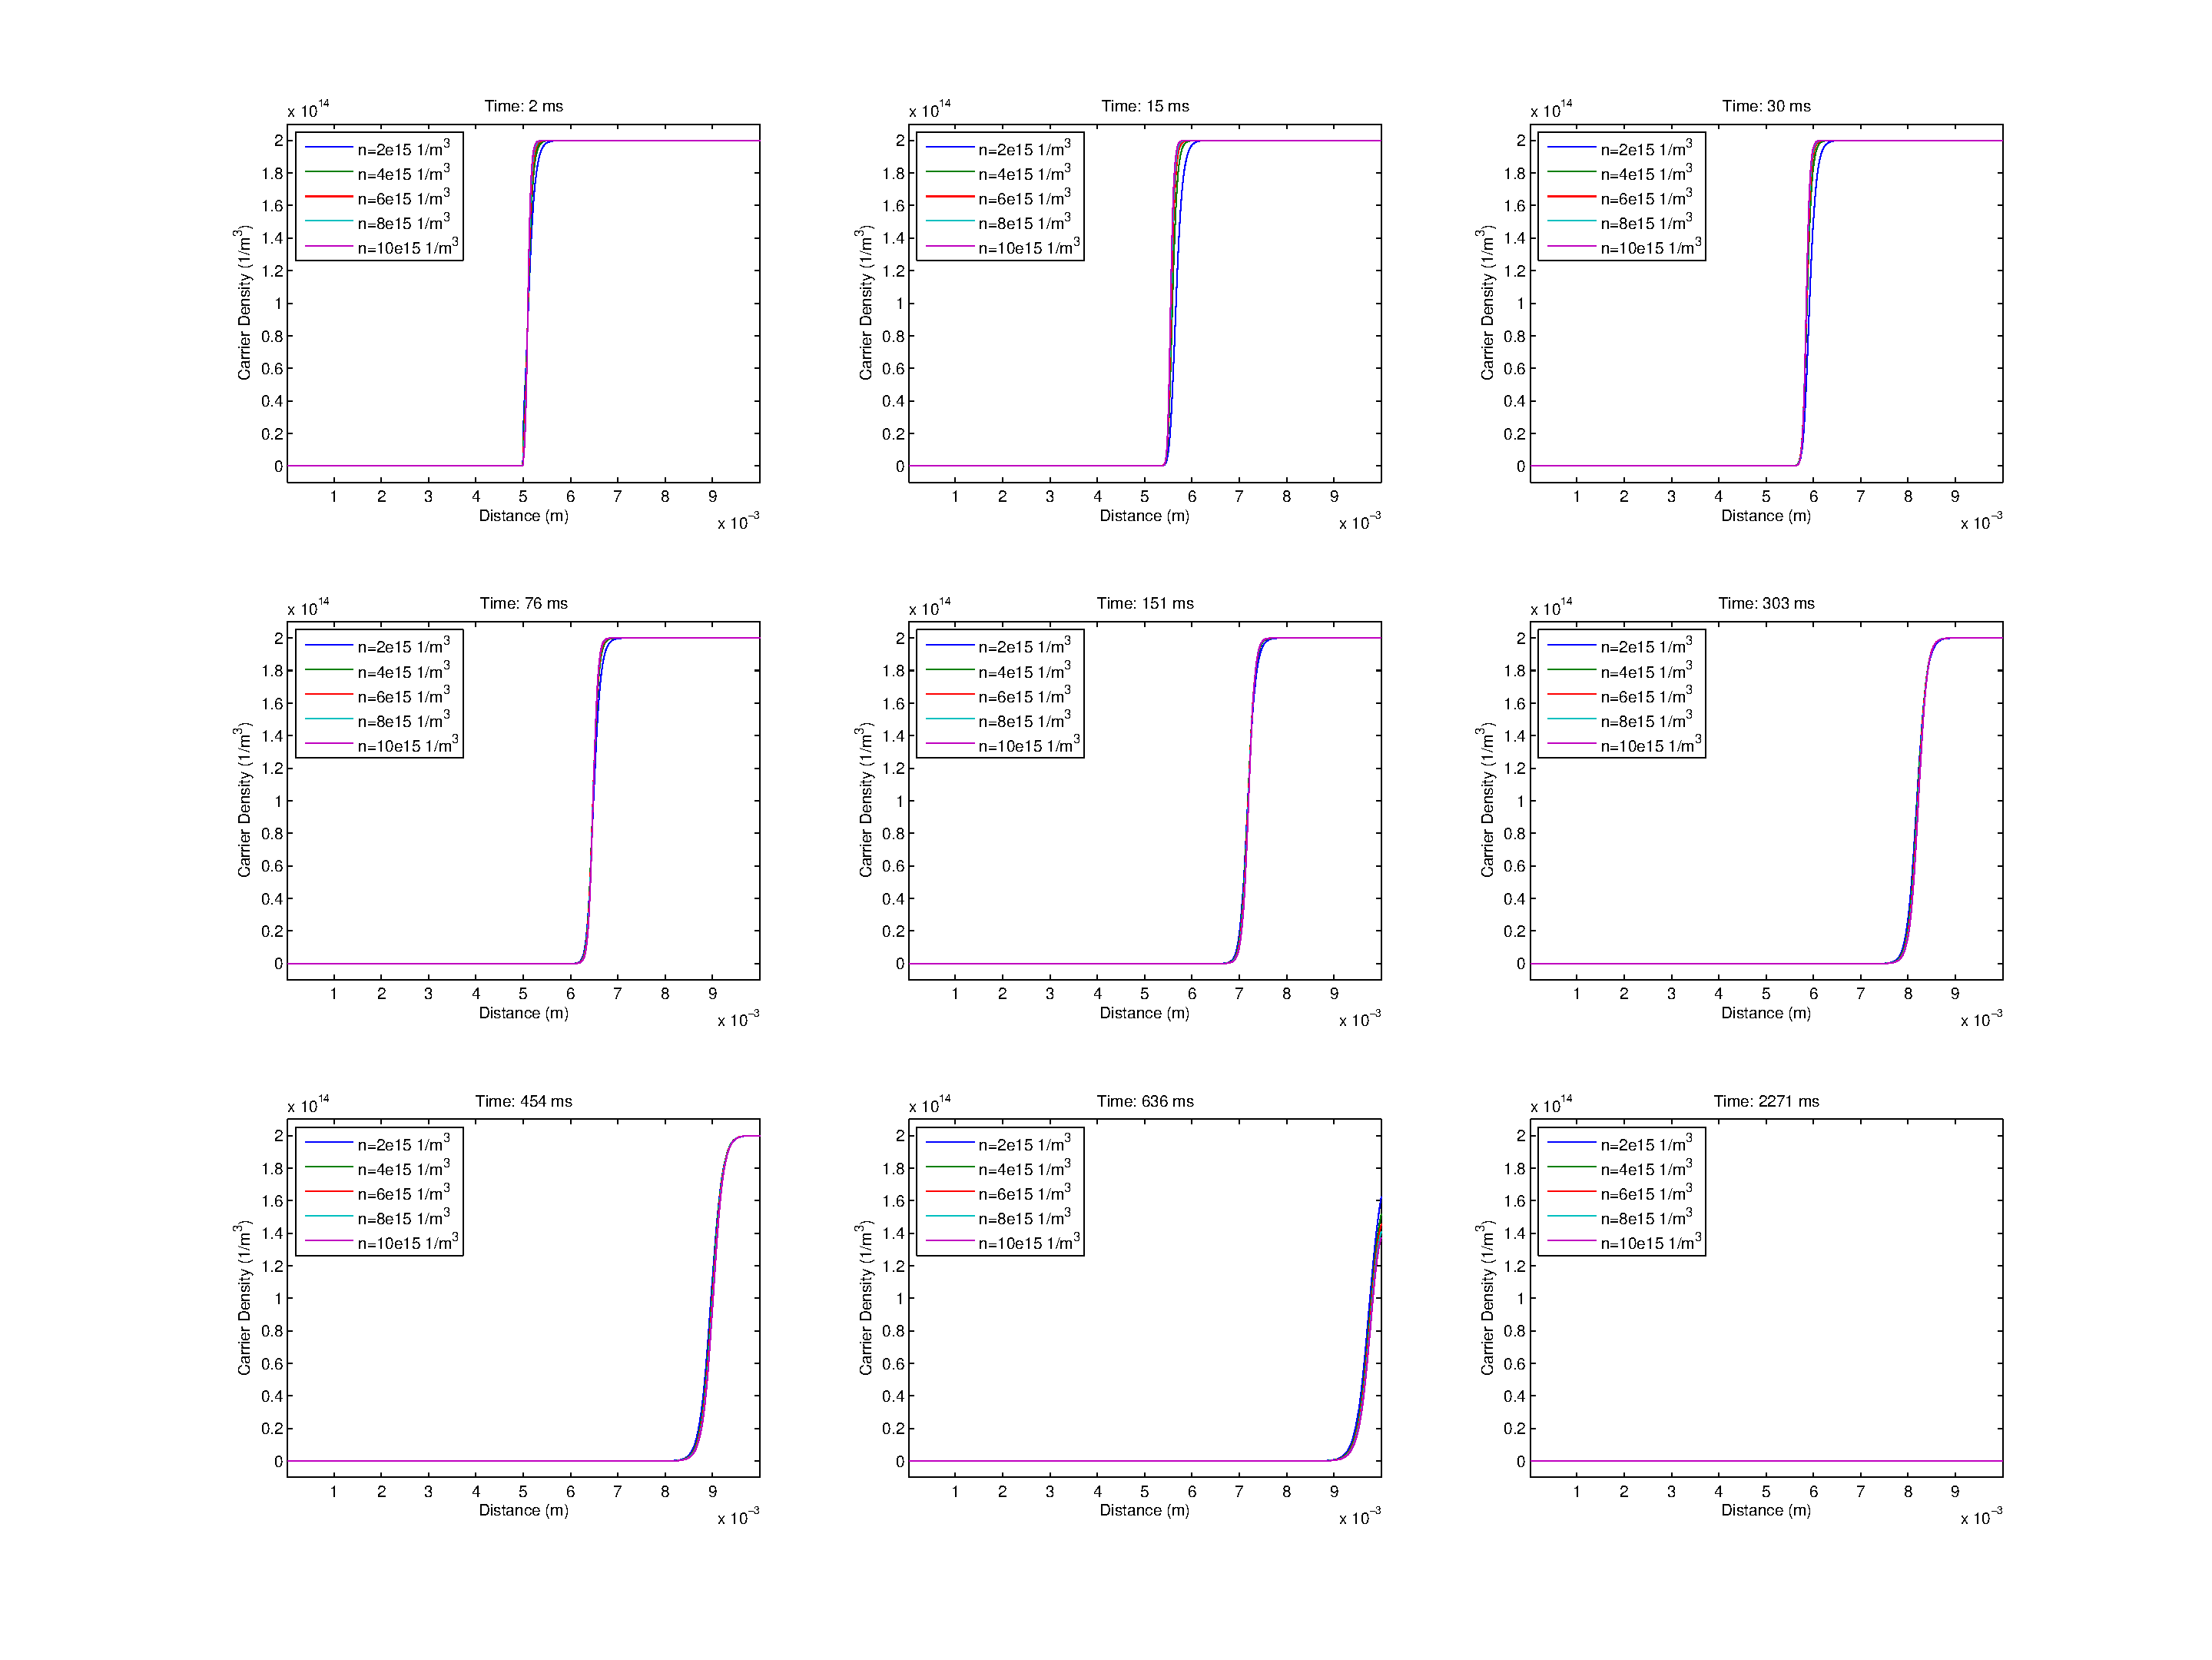
\includegraphics[scale=0.40]{Ex4p_Time}
\caption{Normalized hole distribution over time} 
\label{}
\end{figure}
\end{landscape}
